%%
%% 研究報告用スイッチ
%% [techrep]
%%
%% 欧文表記無しのスイッチ(etitle,eabstractは任意)
%% [noauthor]
%%

%\documentclass[submit,techrep]{ipsj}
%%% <<< SES
%\documentclass[submit,techrep,noauthor]{ipsj}
% \documentclass[submit,ses,noauthor,dvipdfmx]{ipsj}
\documentclass[submit,noauthor,ses,dvipdfmx]{ipsj}
%%% >>> SES


\usepackage[dvips]{graphicx}
\usepackage{latexsym}
\usepackage{indentfirst}
\usepackage{url}	% \url{}コマンド用.URLを表示する際に便利
\usepackage{graphicx}  % ←graphicx.styを用いてEPSを取り込む場合有効にする
\usepackage{color}
\usepackage{listings}
\usepackage{multirow}
% \usepackage{caption} 

\renewcommand\lstlistingname{Program}
\newcommand{\todo}[1]{\colorbox{yellow}{{\bf TODO}:}{\color{red} {\textbf{[#1]}}}}
\newcommand{\done}[1]{\colorbox{green}{{\bf Done}:}{\color{black} {\textbf{[#1]}}}}

\def\Underline{\setbox0\hbox\bgroup\let\\\endUnderline}
\def\endUnderline{\vphantom{y}\egroup\smash{\underline{\box0}}\\}
\def\|{\verb|}


\begin{document}


\title{複数プロジェクトのコード特徴量に基づく\\コーディング規約違反の修正予測精度の評価}

% \etitle{Evaluation of accuracy in predicting fixes for coding convention violations based on code features from multiple projects \\ (version 2024/6/7)}

\affiliate{WU}{和歌山大学\\Wakayama Uniersity, Sakaedani 930, Wakayama-city 640--8510, Japan}


\author{亀岡  令}{Kameoka Ryo}{WU}[s256065@wakayama-u.ac.jp]
\author{伊原  彰紀}{Ihara Akinori}{WU}[ihara@wakayama-u.ac.jp]

\begin{abstract}
OSS開発において複数の開発者がソースコードを読み,理解する必要があるため,ソースコードの可読性は重要である.開発者はコーディング規約に従った実装を行うことによって一定の可動性を担保することができる.
コーディング規約に従っていないコードは,静的解析ツールによって自動的に検出することができるが,大量に検出されるため一部のコードしか修正されないことが多い.
従来研究では,機械学習を用いて予測対象プロジェクトの違反修正履歴を学習することによって,修正優先度予測を行っている.
本研究では,コーディング規約に違反しているソースコードの修正予測を行う際に,予測対象以外の複数のプロジェクトの開発履歴を学習することによる予測精度への影響を調査する.また,提案手法と従来手法で予測精度が大きく変化したプロジェクトにおける予測結果の具体的な差異について分析を行う.


\end{abstract}

\maketitle

%%%%%%%%%%%%%%%%%%%%%%%%%%%
\section{はじめに}
%%%%%%%%%%%%%%%%%%%%%%%%%%%

コーディング規約とは,ソースコードを一定の品質に保つための記述方法について,禁止事項や推奨事項,保守性を高めるためのコーディングスタイルなどを定めたものである.
ソフトウェア開発者はコーディングスタイルの共通化や,ソースコードの最適化のためにコーディング規約を遵守することによって,ソースコードの可読性が向上し,ソフトウェア保守が容易になることが知られている\cite{EffectsSAT}.また,プロジェクトへのコーディング規約の導入によって,ソフトウェア開発におけるソースコードの理解の促進,バグの早期発見などへの効果も確認されている\cite{Beller2}\cite{Johnson}\cite{Beller}.

コーディング規約に違反している箇所を機械的に検出するために静的解析ツールが用いられる.
%静的解析ツールはソースコードを実行することなく,ソースコードに含まれるコーディング規約に違反している箇所を検出することができ,継続的インテグレーションのプロセスの1つとして使用されることも多い.
静的解析ツールは,ソースコード中のコーディング規約に違反しているコード断片を正規表現などにより検出することができ,開発者は静的解析ツールが検出した違反を確認することで,コーディング規約違反箇所を速やかに修正することができる.静的解析ツールは多くの規約の種類を定義しているため,誤検出を含む大量の規約違反検出結果が出力されることが頻繁に発生する.静的解析ツールの誤検出は開発効率の低下につながるため,検出精度を向上させるための研究が行われている\cite{Nguyen}.

従来研究では大量に検出されるコーディング規約違反の中から,優先して修正すべき違反を検出する手法が数多く提案されている\cite{JyuraiPre}
% \todo{引用増やせれば}.
%他にも静的解析ツールの検出結果を優先度づけする研究は数多く行われている.
従来研究の多くは,単一プロジェクトの規約違反修正履歴を学習することで各プロジェクトのコーディングの慣習を捉えた予測を行っているが,単一プロジェクトの規約違反修正履歴のみ学習データとしているため,十分なデータが集まらなかった場合に学習不足に陥ることが考えられる.
そこで,Tabassumらは,不具合予測やソースコードの自動修正において,データ不足,コールドスタート問題への対応として,異なるプロジェクトの開発データを用いることによって学習データを補う手法を提案している\cite{Tabassum}.
ただし,複数プロジェクトのデータを用いることによって,実装方針の異なるプロジェクトのデータを学習することとなるため,十分なデータがある場合には,単一プロジェクトのデータのみを学習したほうが高い予測精度を得ることができる.

本研究では,複数プロジェクトの開発データを予測モデルの学習に使用することによる,コーディング規約違反の修正予測精度への影響を明らかにする.
提案手法として2種類の予測モデルを構築する.1つは,複数プロジェクトのデータを単純に結合し,学習するモデル構築手法である.
もう1つは,複数プロジェクトのデータを結合後にクラスタリングを行い,各クラスタごとに予測モデルを構築する手法である.
本研究の提案手法は,著者らが過去に提案した手法と基本方針は同様である\cite{mine}\cite{mine_live}.しかし,先行研究の手法では学習に利用していたデータセットが小さく,手法の有効性が十分に示されていない.そこで本研究ではデータセットに利用するプロジェクト数を10から68プロジェクトに増加させ,2種類の予測モデルを提案手法として扱う.
また,本研究では先行研究では行っていなかった予測結果の詳細な分析まで行っている.

つづく\ref{chap:background}章では,本研究の位置付け,および従来研究を述べる.\ref{chap:approach}章では,提案手法の詳細な学習データの作成方法や機械学習モデルの作成方法の説明を行う.\ref{chap:result}章では,従来手法である単一プロジェクトのデータのみを学習する手法と提案手法である複数プロジェクトのデータを学習する手法を用いた修正予測を行い,手法ごとのモデルの精度および予測内容の分析を行った結果を示す.\ref{chap:consideration}章では,結果に基づく考察を行い,\ref{chap:heuristic}章では本研究の妥当性への脅威について述べ,\ref{chap:end}章でまとめる.

%%%%%%%%%%%%%%%%%%%%%%%%%%%
\section{コーディング規約と静的解析ツール}\label{chap:background}
%%%%%%%%%%%%%%%%%%%%%%%%%%%

\subsection{コーディング規約違反}


% \begin{figure}[t]
% % \small
% \vspace{-16pt}
%     \begin{lstlisting}[caption={[upper/lower text]%
%                \begin{tabular}[t]{@{}l@{}}
%                 problematic.py \\[1.0\normalbaselineskip]
%                \end{tabular}},frame={tb},numbers=left,label=problematic,identifierstyle={\small}]
% def print_fruits():
%     fruit1 = "orange"
%     fruit2 = "apple" # [unused-variable]
%     print(fruit1)
% \end{lstlisting}
% \vspace{-8mm}

% % \small
%     \begin{lstlisting}[caption={[upper/lower text]%
%                \begin{tabular}[t]{@{}l@{}}
%                 correct.py \\[1.0\normalbaselineskip]
%                \end{tabular}},frame={tb},numbers=left,label=correct,identifierstyle={\small}]
% def print_fruits():
%     fruit1 = "orange"
%     fruit2 = "apple"
%     print(fruit1, fruit2)
% \end{lstlisting}
% % \vspace{-4mm}
% \end{figure}



コーディング規約とは,企業や開発チームのような複数人でプロジェクト開発を行う際に,プログラミングにおける規則についてまとめたものである.
規約の中には変数やクラス,関数などの命名規則について定めたものや,その他に禁止事項,制限事項,推奨事項などが定義されている.
コーディング規約には,コードの構造やコーディングスタイルなどを共通化させるためのルールが定められており,プログラミング言語ごとに複数存在している.例えばPython言語のPEP8,Java言語のCode Conventions for the Java Programming LanguageやGoogle Java Style Guide,JavaScript言語のGoogle JavaScript Style GuideやAirbnb JavaScript Style Guideのようにプログラミング言語ごとに違反の`種類'や`基準'が異なる規約が複数存在する.

% 次にコーディング規約への違反の例とその修正例を示す.Program \ref{problematic},\ref{correct}はPythonのコーディング規約PEP8に違反しているコードと修正した例である.
% また,静的解析ツールのPylintの公式文書であるPylint 2.17.5 documentation\footnote{https://pylint.readthedocs.io/en/stable/index.html}に掲載されているコーディング規約への違反・修正例である.
% ここで掲載している違反はソースコード中に利用されていない変数が宣言されている場合に検出される違反である.
% Program \ref{problematic}で宣言されている変数\texttt{`fruit2'}は利用されておらず,利用するように修正したコードがProgram \ref{correct}である.この例では\texttt{`fruit2'}を削除することでも解消される.

コーディング規約違反の検出は開発者が目視で行うには多くのコストを要するため,静的解析ツールが用いられる.静的解析ツールにも各言語ごとに複数の種類があり,参照している規約の種類や,違反を検出した際のメッセージのフォーマットや,検出する違反のカスタマイズ性の高さなどが異なる.

% \subsection{静的解析ツールの問題点}

%静的解析ツールを用いて開発するには問題点が存在する.
静的解析ツールは各違反ごとに定められたルールに合致した場合にすべて違反として検出し出力するため,大量の検出結果が出力されることが頻繁に発生する.実際に多くのプロジェクトで,静的解析ツールが大量の規約違反を検出することが多いことを従来研究で明らかにしている\cite{UsingStaticAnalysisTools2}.
大量の違反の検出結果には誤検出も含まれ,それらを開発者がレビューし修正するには多くのコストを要するため困難である.
さらに様々な違反から優先して修正すべき規約違反を特定することは,開発の経験や,複雑なソースコードの理解が必要であるため,共同開発者において容易でない\cite{shuseisarenai}.


\subsection{従来研究}

従来研究では
%各プロジェクトごとに異なる優先して修正すべき規約違反の特定のために,機械学習モデルを用いた特定手法などが数多く提案されている.
静的解析ツールの誤検出を含む大量の検出結果によって開発効率の低下を防ぐため,Ruthruffらは機械学習モデルを用いて優先して修正すべき違反を特定する手法を提案している\cite{JyuraiPre}.
Kimらは静的解析ツールの出力結果をベイジアンネットワークに活用することにより,規約違反しているコードの修正優先度の予測を行う手法が提案されている\cite{beizu}.
これらの研究のほかにも静的解析ツールによって検出された規約違反コードの修正優先度付けを行う研究や,修正の要否を予測する研究は数多く行われている\cite{Wang}\cite{Qing}\cite{HowFar}.
機械学習のモデル構築には,規約違反コードの優先度予測対象のプロジェクトの過去の規約違反修正履歴を学習データとし,新しいデータを評価用データとすることで構築したモデルの評価を行っている.

従来手法では,予測対象とするプロジェクトの過去の規約違反修正履歴を学習データとして,予測モデルを構築している.各プロジェクトにはコーディングスタイルなどが存在し,修正の要否はプロジェクトごとに異なるため,評価用データと同じプロジェクトのデータを学習するほうが,他プロジェクトのデータを学習するより高い予測精度が得られると考えられる.
しかし,評価用データと同じプロジェクトを学習データとする場合,出現する規約違反の種類や,各違反の修正率が大きく異なる\cite{Panichella}.そのため,規約違反が修正される(正例)と修正されない(負例)の数が不均衡になる場合や,データサイズが小さいことにより,十分な学習ができず予測精度が低下することが示唆される.

本研究では,予測モデルの構築の際に用いる学習データに評価用データとは異なる別プロジェクトの規約違反修正履歴を用いることによる,規約違反コードの修正要否の予測精度への影響を明らかにする.
名倉らは,複数プロジェクトを用いてコーディング規約違反の発生の増減の予測を行っているが,発生した違反が修正されるか否かを予測することは行っていないため,予測の点において本研究との差分となっている\cite{nagura}.
複数プロジェクトの修正履歴データを用いて学習データサイズの拡張を図ることにより,予測精度の向上を期待できるが,他プロジェクトで修正される規約が予測精度の向上に寄与するとは限らない.
%コーディング規約違反の修正予測において複数プロジェクトの規約修正履歴を学習する手法は従来では行われておらず,他プロジェクトの開発データを用いることによって予測プロジェクトとは関係のない規約修正履歴を学習することとなるので予測精度が低下する恐れがある.
そこで,本研究では複数プロジェクトの開発データを学習した場合の予測精度への影響を明らかにすることを目的とする.

%%%%%%%%%%%%%%%%%%%%%%%%%%%
\section{修正を要する規約違反ソースコードの特定手法}\label{chap:approach}
%%%%%%%%%%%%%%%%%%%%%%%%%%%

\subsection{概要}

\begin{figure*}[t]
	\centering
     % 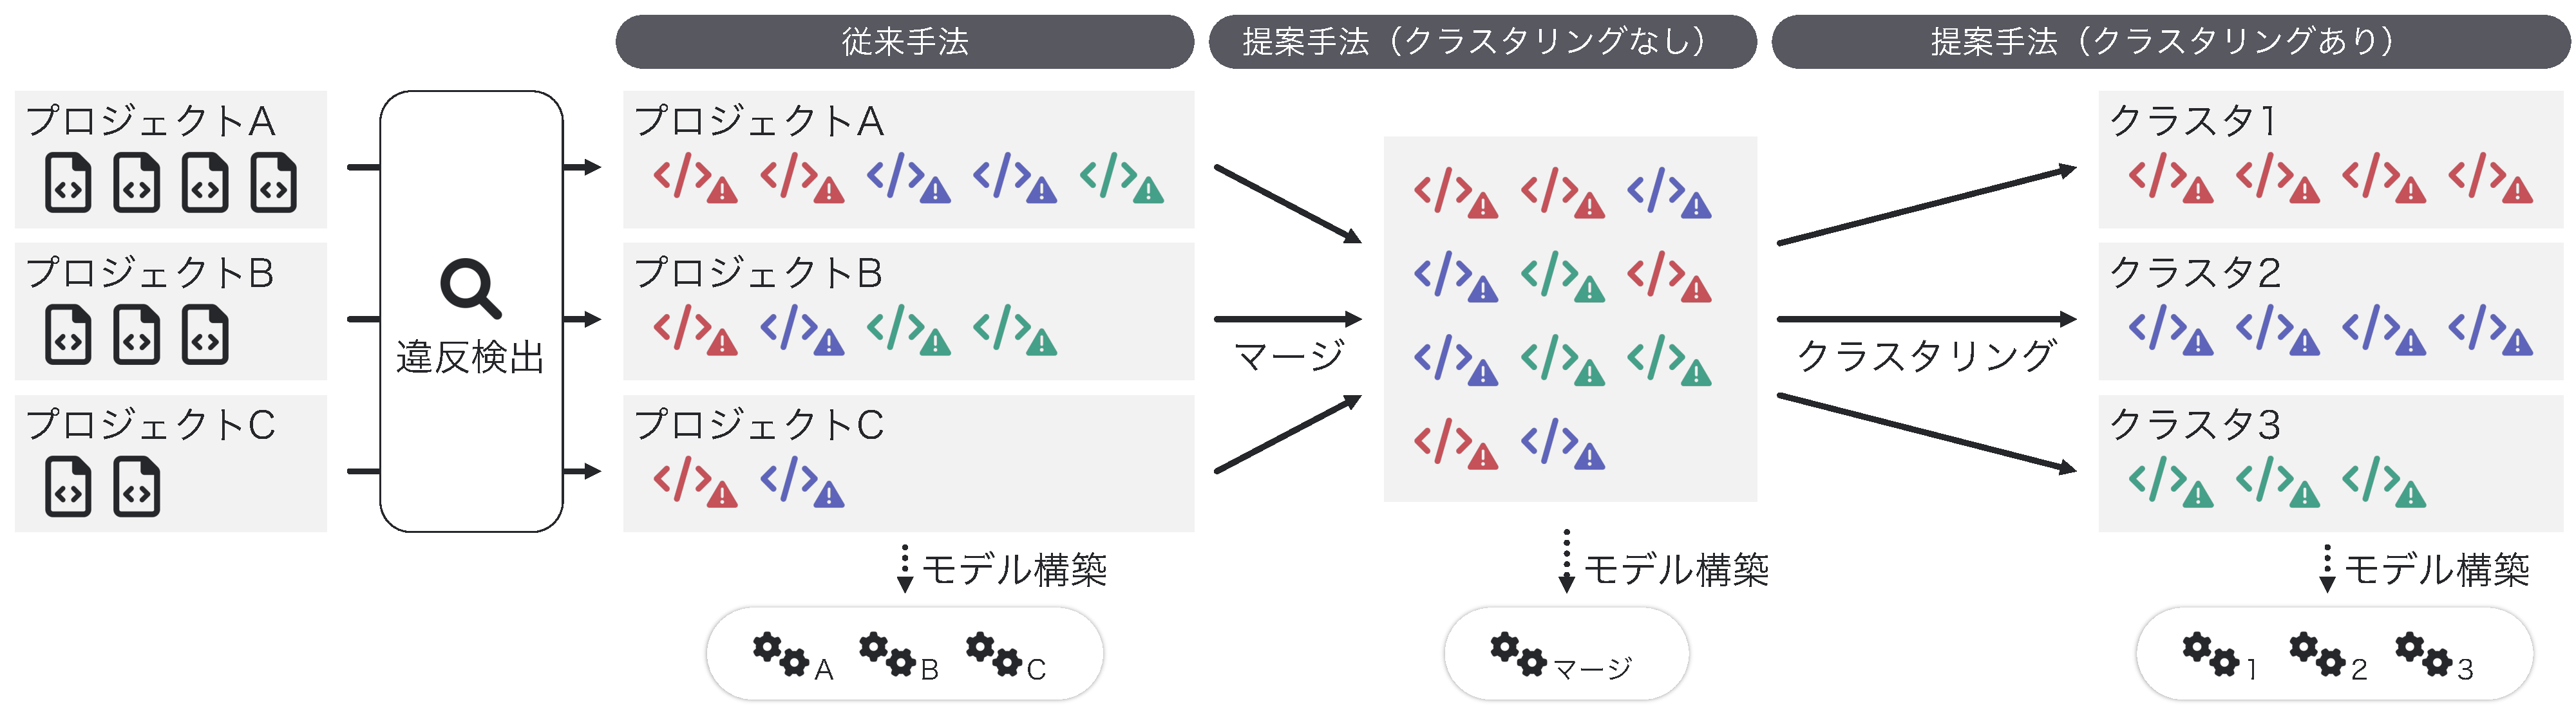
\includegraphics[width=0.5\textwidth, bb=0 0 4 3]{Kameoka_fig/kameoka_fig1.pdf}
	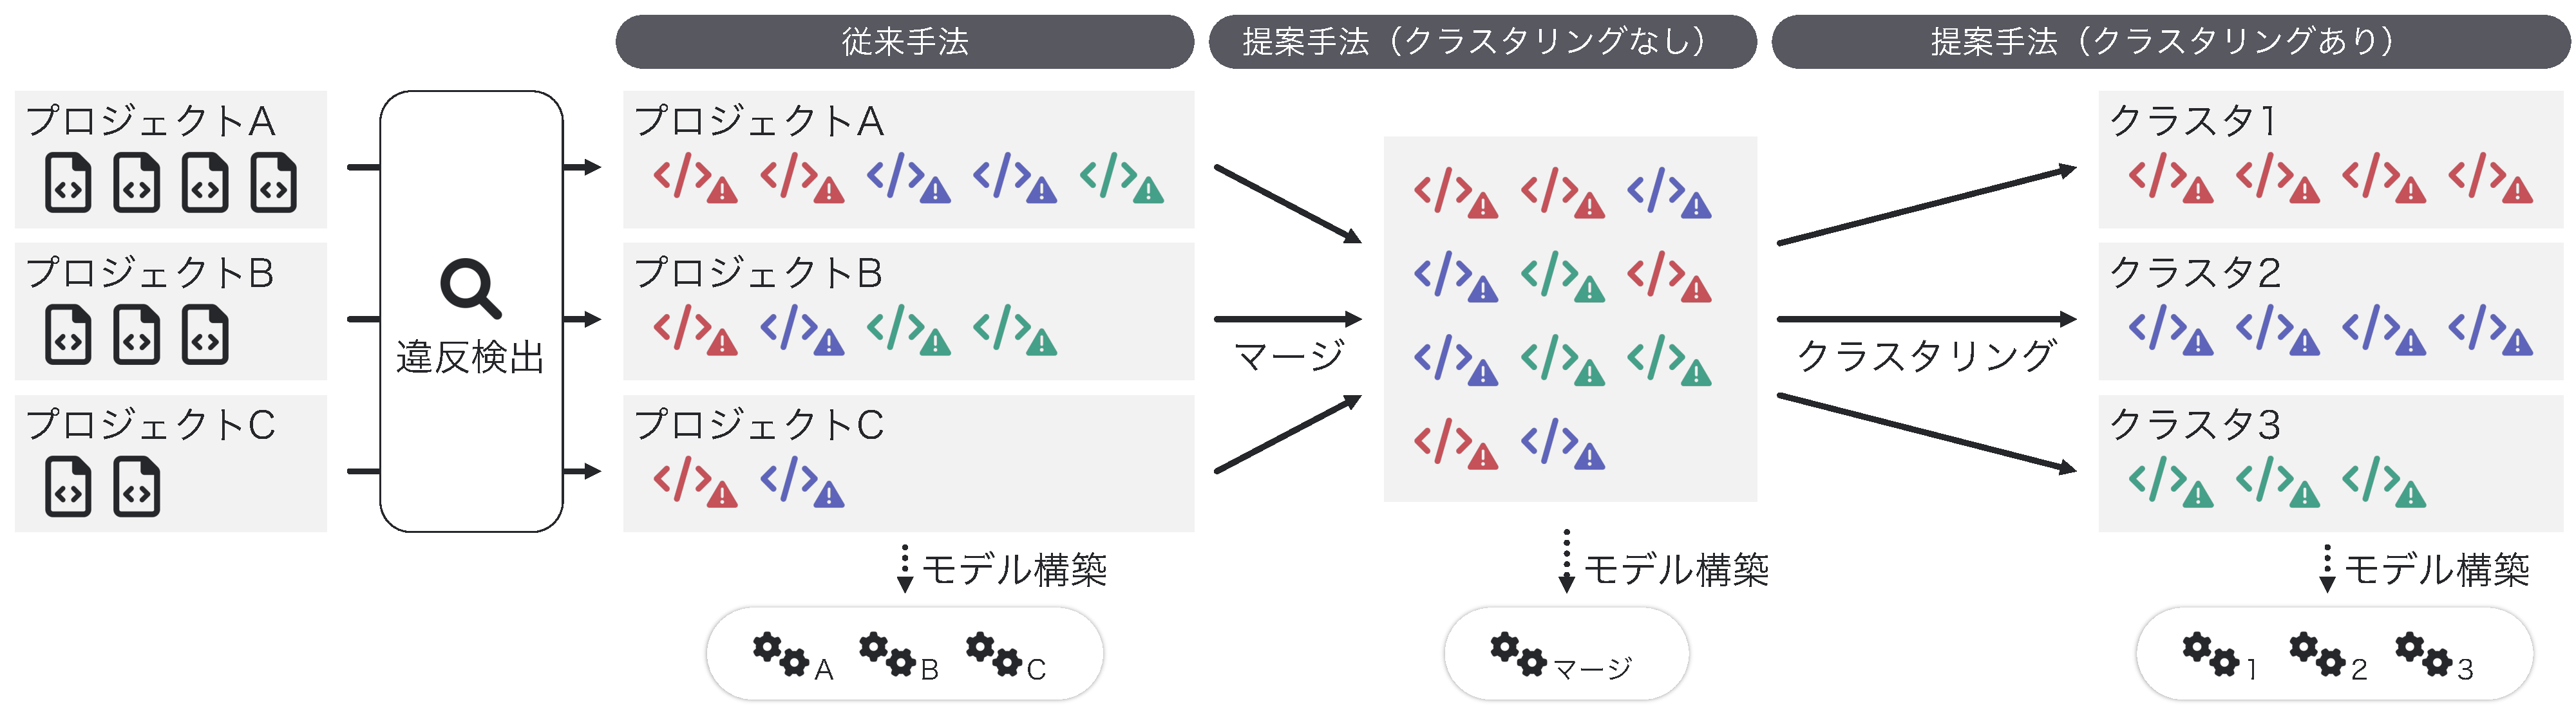
\includegraphics[width=0.8\linewidth]{Kameoka_fig/kameoka_fig1.pdf}
	\caption{本研究の概略図}
	\label{fig:Teiannsyuhou}
\end{figure*}

図\ref{fig:Teiannsyuhou}は本研究の検証手法を示す.本研究では,静的解析ツールによって検出されたコーディング規約違反を修正すべき違反かそうでない違反かの2値に分類する機械学習モデルを3種類作成する.%各モデルの概要は以下の通りである.

\begin{enumerate}
  \item 従来手法:従来研究の手法を採用したモデルであり,予測対象のプロジェクトの過去の規約違反修正履歴のみを学習する予測モデルを構築
  \item 提案手法(クラスタリングなし):提案手法の複数プロジェクトの規約違反修正履歴を学習させる手法で,すべての学習データを結合し学習する予測モデルを構築
  \item 提案手法(クラスタリングあり):提案手法で複数プロジェクトのデータを結合した後に,クラスタリングを行い各クラスタごとに学習する予測モデルを構築
\end{enumerate}


モデル(3)において結合したデータをクラスタリングする理由を説明する.提案手法(クラスタリングなし)では,学習データに複数プロジェクトのデータを用いることによって学習データを拡張しており,各プロジェクトごとに存在するコーディングスタイルなどの特徴を無視したまま結合している.
クラスタリングすることによって,説明変数が類似した違反修正データ群を収集することができるため,すべてのコーディング規約違反修正データを学習するより,類似性を持った説明変数から学習することができる.
クラスタリングによって説明変数が類似し同じクラスタに分類されたプロジェクト同士が,コーディングスタイルも類似するとは言えないが,単純に結合した場合より効果的に複数プロジェクトのデータを学習できると考えられるため,クラスタリングを用いた手法を採用した.



\subsection{学習データと評価データの収集}

本研究では,複数プロジェクトのデータを学習するにあたって,すべてのプロジェクトのデータを学習に用いるために,各プロジェクトのデータを時系列順に並べた際の古いものから8割を学習に用い,残りの2割を検証用データとして用いた.ここで時系列順に並べている理由は,学習時に未来のデータを学習させないために時系列の古いものを学習データとするためである.そのため,モデルの評価時に,交差検証は行わない.時系列を考慮した時系列十分割交差検証という手法も存在するが,データサイズが小さいプロジェクトでは,学習データサイズが小さくなりすぎることが危惧されるため,時系列十分割交差検証も行わない.



\subsection{説明変数・目的変数の計測方法}


%-------------------------
\begin{figure}[t]
	\centering
	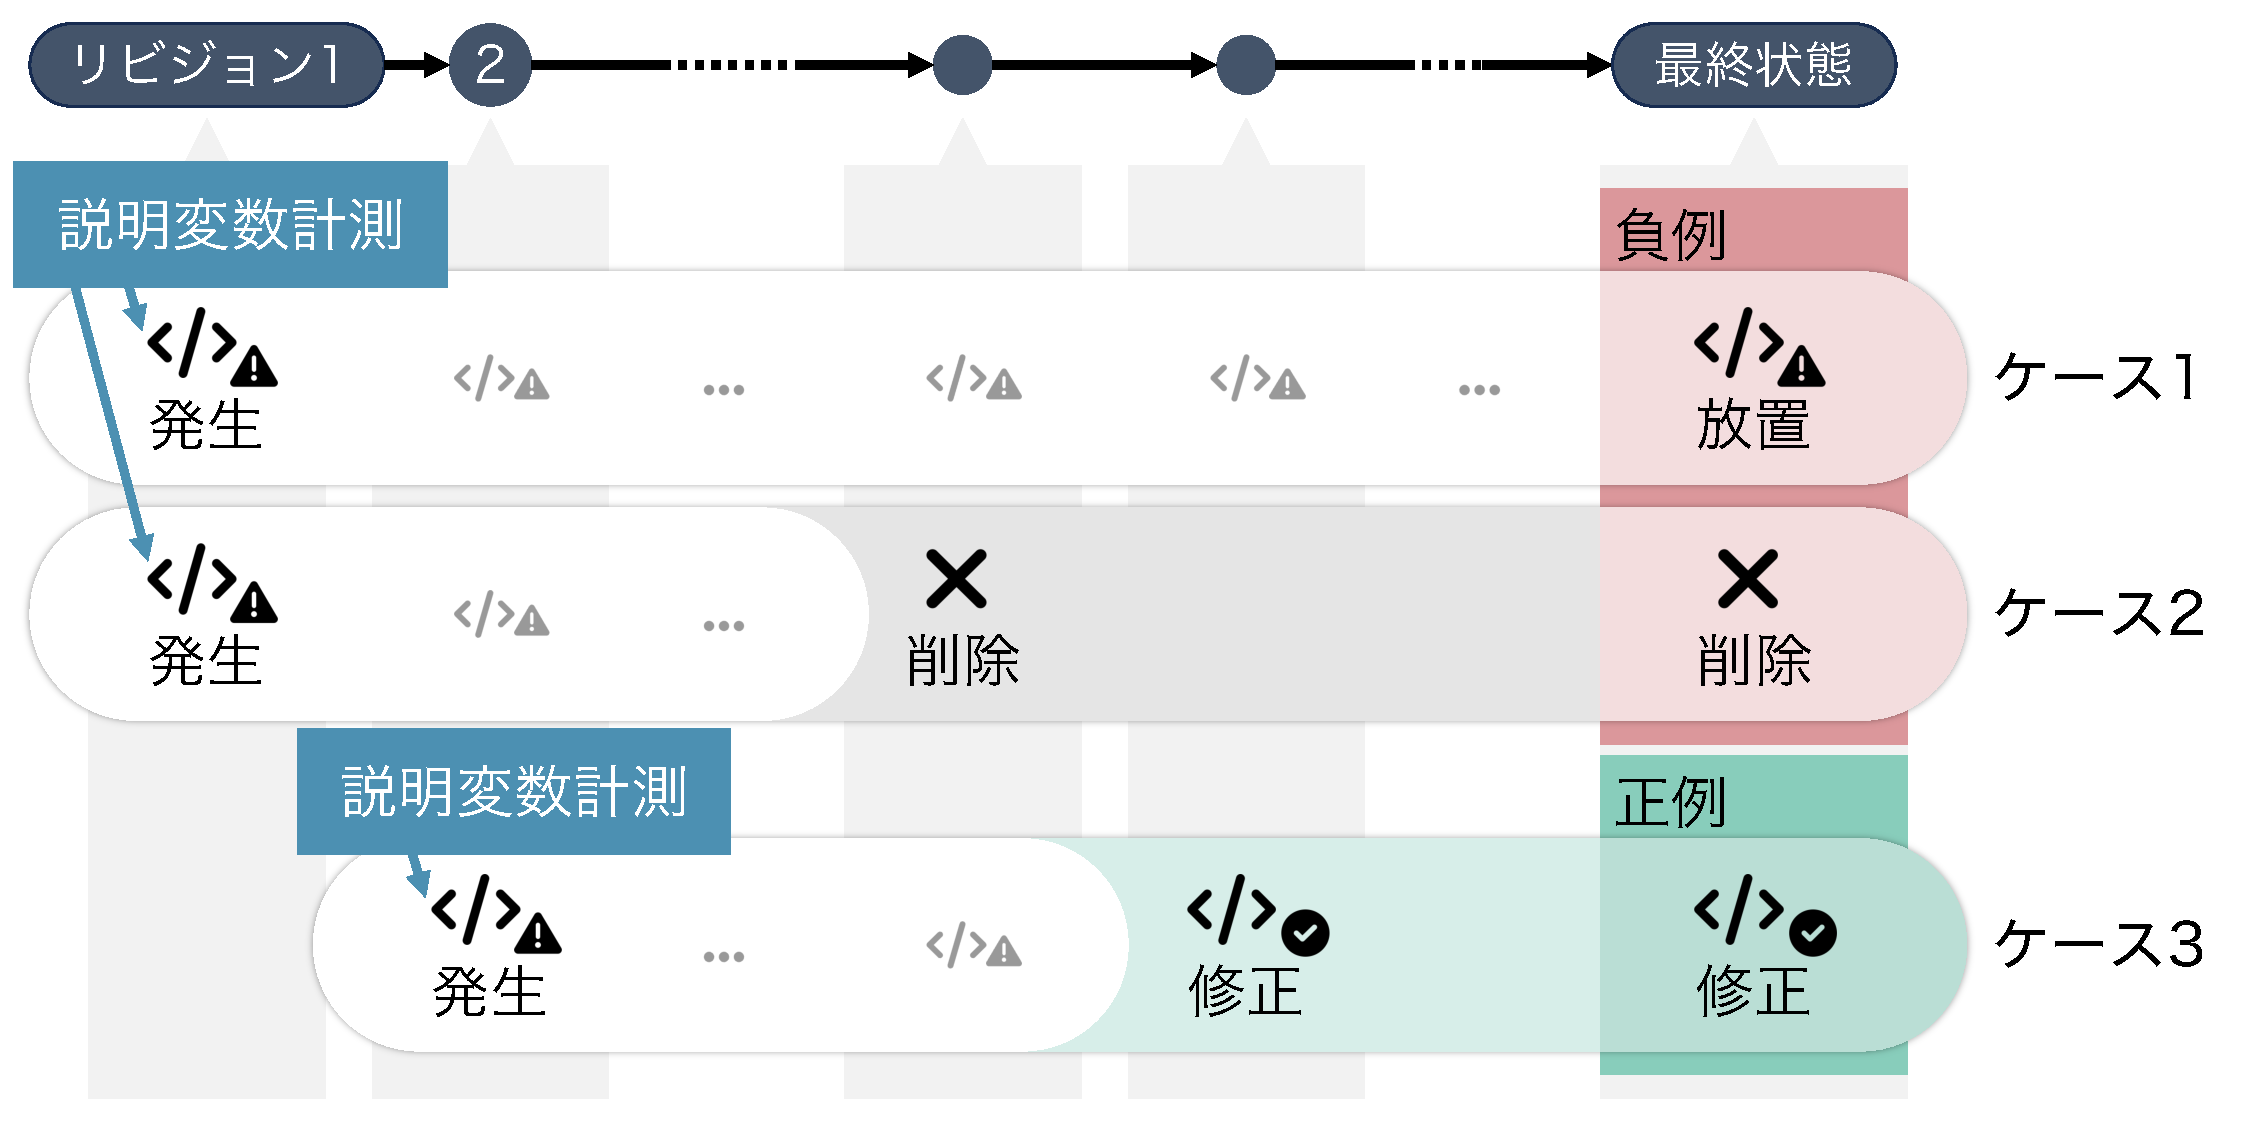
\includegraphics[width=1.0\linewidth]{Kameoka_fig/kameoka_fig2.pdf}
    % 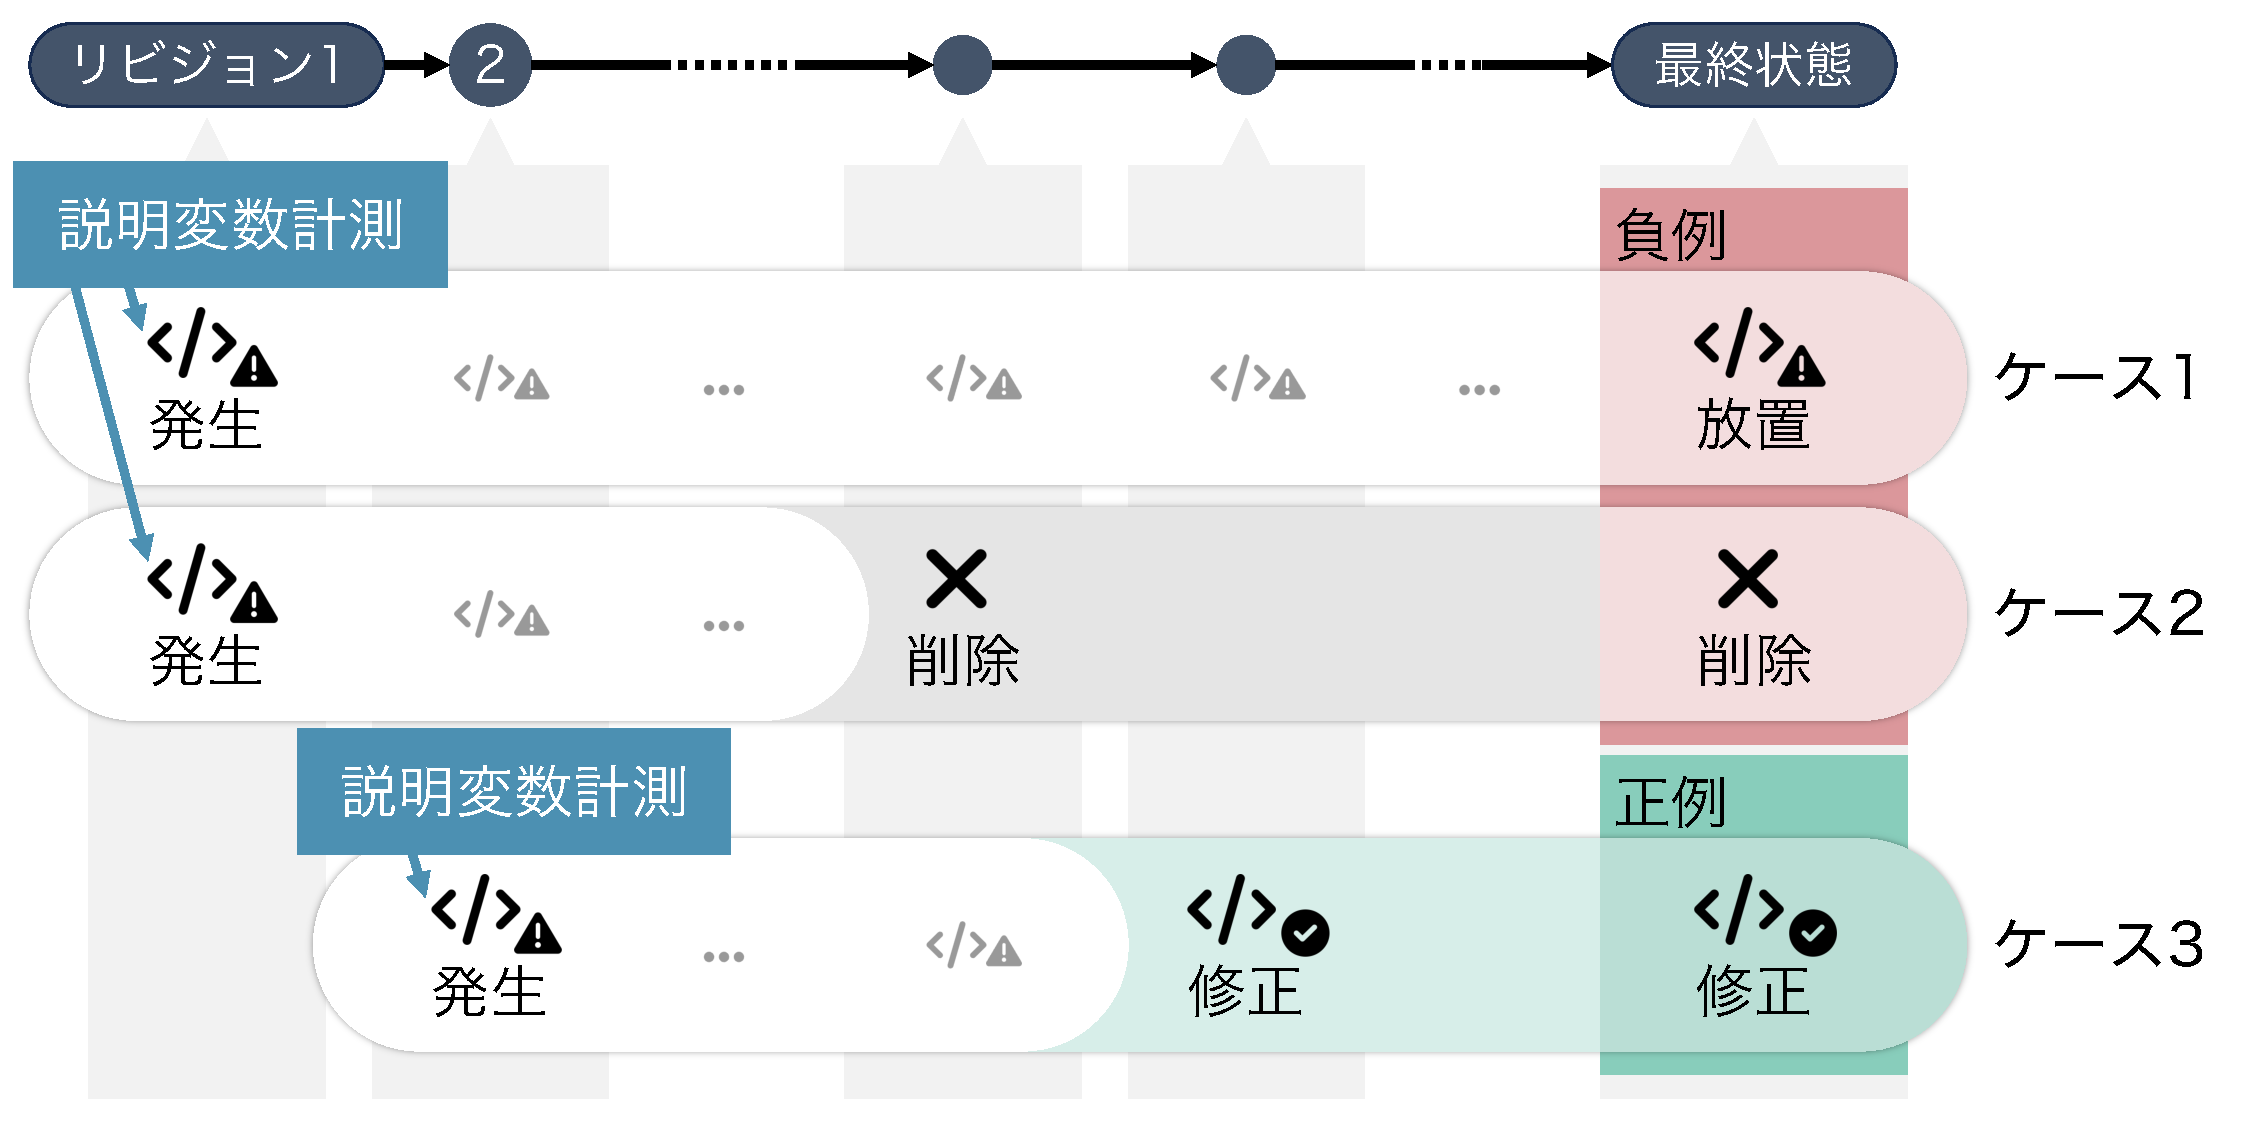
\includegraphics[width=0.25\textwidth, bb=0 0 4 3]{Kameoka_fig/kameoka_fig2.pdf}
	\caption{説明変数と目的変数の計測方法}
	\label{fig:mokutekihensu}
\end{figure}
%-------------------------

図\ref{fig:mokutekihensu}は,本研究における説明変数と目的変数の計測位置と,計測方法を示す.本研究では,規約違反修正履歴から静的解析ツールによって初めて違反が検出された場所を説明変数の計測地点とし,最終状態において,各違反が修正されたか否かによって目的変数を計測する.
目的変数の計測についてケースごとにまとめたものが表\ref{tab:pos_neg}である.
図\ref{fig:mokutekihensu}と表\ref{tab:pos_neg}に示すケース1からケース3はそれぞれ対応する同じ事象を示す.
説明変数は,ソースコードの特徴量であるコード行数,コメント行数,循環的複雑度などを含むソースコードに関する特徴量43種類に,コーディング規約違反IDをOne-hotベクトル化した1種類の,合計44種類の特徴量を使用する.コーディング規約に違反するコード断片を含むソースコードファイルの関数,クラス,モジュールに対して特徴量をテクマトリックス株式会社が開発する静的解析ツールUnderstand
% \footnote{Understand:\url{https://www.techmatrix.co.jp/product/understand/}}
を用いて計測する.

%すべての計測したコーディング規約違反は表の3種類に分類され,目的変数を計測し,各違反の発生地点において説明変数を計測する.



%----------------------
\begin{table}[t]
    \centering
    \caption{正例と負例の分類}
    \label{tab:pos_neg}
    \scalebox{0.85}{
    \begin{tabular}{l|l}
         \hline
            分類 & 説明\\ \hline
            負例(ケース1) & コーディング規約の違反が放置されているコード断片\\
            負例(ケース2) & コーディング規約に違反していたコード断片が削除された\\
            正例(ケース3) & コーディング規約に違反していたコード断片が修正された\\
         \hline
    \end{tabular}
    }
\end{table}
%-----------------------

\subsection{コーディング規約に違反しているコード断片のクラスタリング}


提案手法(クラスタリングあり)において,説明変数の特徴量が類似しているコード断片をクラスタリングし,各クラスタごとに予測モデルを構築する.クラスタリングには,クラスタ間の類似度を計測するため階層的クラスタリングを用いる.階層的クラスタリングには,連結法としてWard法を用い,距離の測定にはユークリッド距離を用いる\cite{ward}.本研究ではクラスタ数を10とした場合における結果を用いて評価を行う.
最適なクラスタ数の決定には決定問題が伴うが,本研究ではデータ数が非常に多く最適なクラスタ数を決定することが困難なため,暫定でクラスタ数を10としている.


\subsection{機械学習モデルの構築と評価}

本研究で利用する予測モデルは,機械学習の予測手法として頻繁に利用されるロジスティック回帰,RandomForestの2種類の手法を用いる.
本研究で用いたデータセットに含まれるプロジェクトごとの違反修正率の中央値は0.36であった.つまり,コーディング規約違反の修正に関するデータは,違反が修正された正例が少なく,修正されない負例が多い不均衡なデータであるため,各予測モデルを構築するためのPythonパッケージに用意されているオプションであるclass\_weightsを用いることによって,2クラスデータに重みづけを行う.
また,学習の反復回数を定めるイテレーション回数を10,000に設定する.
% 構築した各予測モデルの評価には,従来研究でも用いられていた適合率,再現率,F1値を使用する.

%%%%%%%%%%%%%%%%%%%%%%%%%%%
\section{評価実験}\label{chap:result}
%%%%%%%%%%%%%%%%%%%%%%%%%%%

\subsection{データセット}

\begin{figure}[t]
	\centering
    % 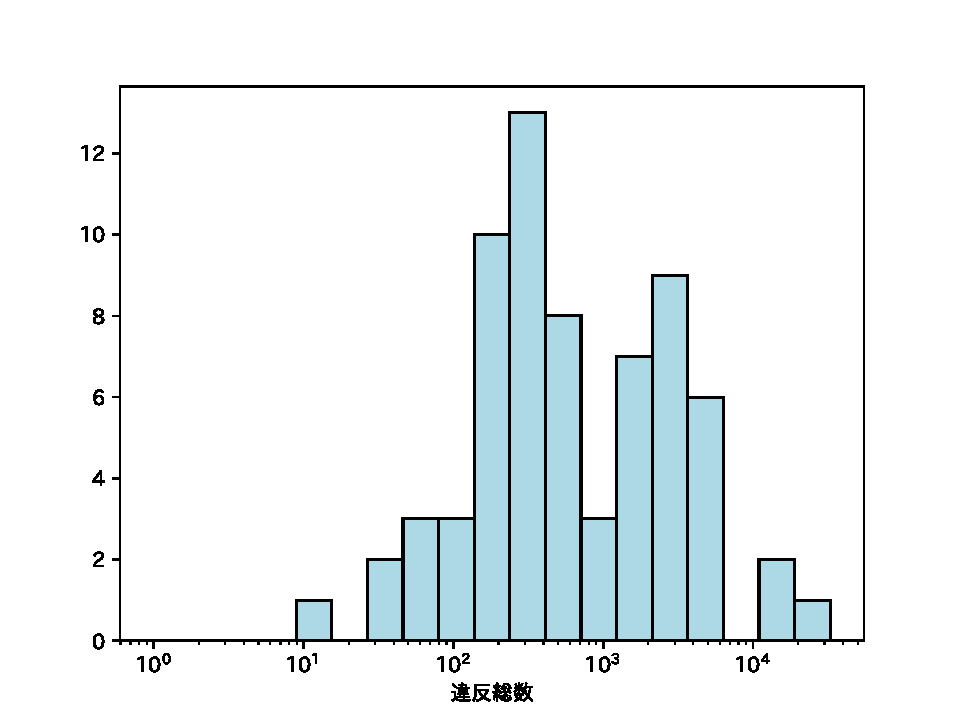
\includegraphics[width=0.25\textwidth, bb=0 0 4 3]{Kameoka_fig/dataset_hist.pdf}
	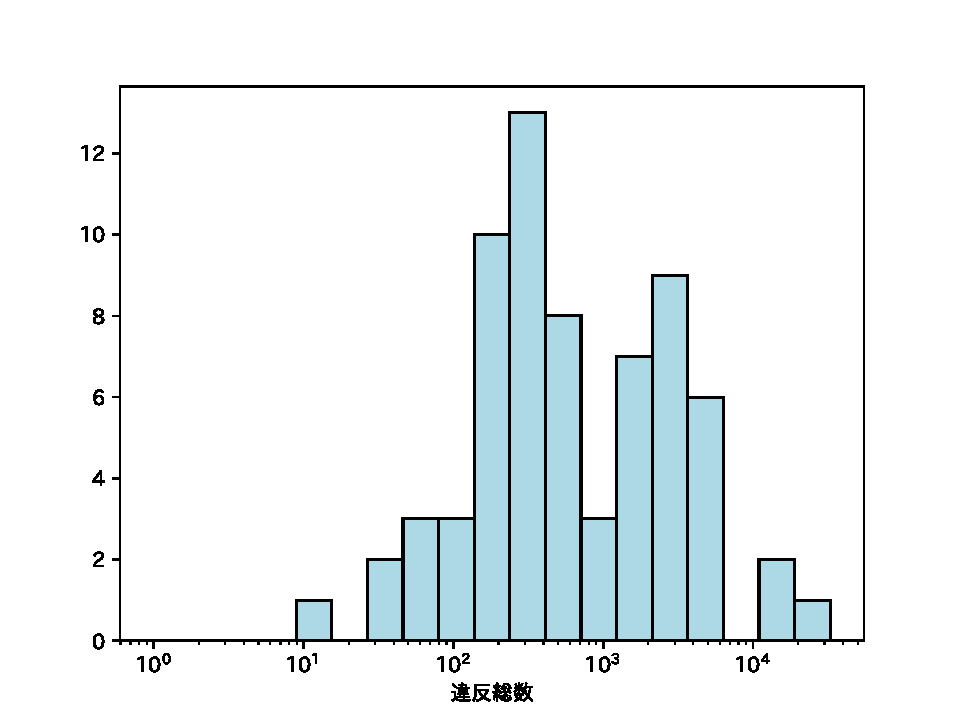
\includegraphics[width=1\linewidth]{Kameoka_fig/dataset_hist.pdf}
	\caption{データセットに含まれるプロジェクトごとの違反総数のヒストグラム}
	\label{fig:dataset}
\end{figure}

\subsubsection{対象プロジェクトの選定方法}
本研究ではケーススタディとして,OSSライブラリ検索サービスであるLibraries.io\footnote{Libraries.io: \url{https://libraries.io/}}からPython言語で実装され,静的解析ツールPylintを開発に使用しており,GitHubにソフトウェア,および規約違反修正履歴を公開しているプロジェクトを対象とする.
特に,Libraries.ioにおいてOSSの人気度合いや活発度合いを示すSourceRankの上位1,500プロジェクトから静的解析ツールの設定ファイル(pylintrc,または.pylintrc)を保有する81プロジェクトの内,取得した目的変数を学習用データと検証用データに分割した際に,どちらのデータにも正例と負例を含む68プロジェクトを対象とする.

本研究では,各分析対象プロジェクトにおいて,2018年12月から1,000日間のコミット履歴を分析対象とする.図\ref{fig:dataset}に,各プロジェクトの総コーディング規約違反数をヒストグラムで示す.図の横軸はプロジェクトごとの総違反数対数軸で示す.違反数が100から1,000のプロジェクトが最も多い.

% \subsubsection{対象プログラミング言語の選定理由}

% Python言語は,近年のLLM(大規模言語モデル)をはじめとする機械学習技術の開発・利用に頻繁に用いられている.また,Pythonはデータ分析においても充実したライブラリが存在し,その有用性が広く知られている.よって,本研究ではPython言語を対象言語として選択した.

% \subsubsection{静的解析ツールの選定理由}

% 本研究で分析対象とする静的解析ツールにはPylintを選定した.Pylintは他の静的解析ツールより多くのコーディング規約が設定されていることが特徴である.Python言語のコーディング規約であるPEP8に基づいた静的解析ツールは数多く存在するが,Pylintは設定ファイルによるスタイルチェックや論理エラーチェックの対象を柔軟にカスタマイズすることができ,Pythonの代表的な静的解析ツールのflake8より厳しい判定基準を設けている.
% Pylintは他の静的解析ツールより豊富なルールでコーディング規約違反を検出することができ,ソースコードから4カテゴリに分類される多くの違反を検出できるため本研究での対象静的解析ツールとして選択した.

\subsection{RQ1: 複数プロジェクトのデータ用いることで予測精度は向上するか?}

% \subsubsection{実験結果}

\begin{table*}[t]
    \centering
    \caption{各手法による評価指標で最も高い値で予測したプロジェクト数の一覧}
    \label{tab:gen}
    \scalebox{0.9}{
            \begin{tabular}{l|p{7em}p{7em}p{7em}|p{7em}p{7em}p{7em}}
            \hline
            \multirow{2}{*}{手法}&\multicolumn{3}{c|}{{ロジスティック回帰}} & \multicolumn{3}{c}{RandomForest} \\ \cline{2-7}
             & \multicolumn{1}{r}{{適合率}} & \multicolumn{1}{r}{{再現率}} & \multicolumn{1}{r|}{{F1値}} & \multicolumn{1}{r}{{適合率}} & \multicolumn{1}{r}{{再現率}} & \multicolumn{1}{r}{{F1値}} \\ \hline
            従来手法 & \multicolumn{1}{r}{{48}} & \multicolumn{1}{r}{{27}} & \multicolumn{1}{r|}{{38}} & \multicolumn{1}{r}{{28}} & \multicolumn{1}{r}{{43}} & \multicolumn{1}{r}{{37}} \\
            % 提案手法(クラスタリングなし) & 12 & 40 & 18 & 27 & 35 & 23 & 17 & 25 & 18 \\
            提案手法(クラスタリングなし) & \multicolumn{1}{r}{{12}} & \multicolumn{1}{r}{{40}} & \multicolumn{1}{r|}{{18}} & \multicolumn{1}{r}{{27}} & \multicolumn{1}{r}{{35}} & \multicolumn{1}{r}{{23}} \\
            % 提案手法(クラスタリングあり) & 20 & 22 & 19  & 28 & 24 & 16 & 24 & 36 & 26 \\ \hline
            提案手法(クラスタリングあり) & \multicolumn{1}{r}{{20}} & \multicolumn{1}{r}{{22}} & \multicolumn{1}{r|}{{19}}  & \multicolumn{1}{r}{{28}} & \multicolumn{1}{r}{{24}} & \multicolumn{1}{r}{{16}} \\ \hline
            % 重複数 & 12 & 21 & 7 & 15 & 34 & 8 & 9 & 17 & 4 \\ \hline
            重複数 & \multicolumn{1}{r}{{12}} & \multicolumn{1}{r}{{21}} & \multicolumn{1}{r|}{{7}} & \multicolumn{1}{r}{{15}} & \multicolumn{1}{r}{{34}} & \multicolumn{1}{r}{{8}} \\ \hline
        \end{tabular}
    }
% \end{table*}
\vspace{3mm}
% \begin{table*}{}
    \centering
    \caption{ロジスティック回帰モデルでの予測結果(総違反数の上位5件を掲載)}
    \label{tab:logistic}
    %\vspace{3mm}
    \scalebox{0.9}{
        \begin{tabular}{l||p{4em}|p{4em}|p{4em}||p{4em}|p{4em}|p{4em}||p{4em}|p{4em}|p{4em}}
            \hline
            \multirow{3}{*}{プロジェクト名}&\multicolumn{3}{c||}{\multirow{2}{*}{従来手法}} & \multicolumn{3}{c||}{提案手法} & \multicolumn{3}{c}{提案手法}\\
            &\multicolumn{3}{c||}{} & \multicolumn{3}{c||}{(クラスタリングなし)} & \multicolumn{3}{c}{(クラスタリングあり)}\\ \cline{2-10}
            & 適合率 & 再現率 & F1値 & 適合率 & 再現率 & F1値 & 適合率 & 再現率 & F1値 \\ \hline
            sockeye & \multicolumn{1}{r|}{\textbf{0.53}} & \multicolumn{1}{r|}{\textbf{0.81}} & \multicolumn{1}{r||}{\textbf{0.64}} & \multicolumn{1}{r|}{0.35} & \multicolumn{1}{r|}{0.56} & \multicolumn{1}{r||}{0.43} & \multicolumn{1}{r|}{0.49} & \multicolumn{1}{r|}{0.67} & \multicolumn{1}{r}{0.57} \\
            coretools & \multicolumn{1}{r|}{\textbf{0.04}} & \multicolumn{1}{r|}{0.63} & \multicolumn{1}{r||}{\textbf{0.07}} & \multicolumn{1}{r|}{0.02} & \multicolumn{1}{r|}{\textbf{0.88}} & \multicolumn{1}{r||}{0.04} & \multicolumn{1}{r|}{0.03} & \multicolumn{1}{r|}{0.83} & \multicolumn{1}{r}{0.05} \\
            howdoi & \multicolumn{1}{r|}{\textbf{0.64}} & \multicolumn{1}{r|}{\textbf{0.99}} & \multicolumn{1}{r||}{\textbf{0.78}} & \multicolumn{1}{r|}{0.12} & \multicolumn{1}{r|}{0.33} & \multicolumn{1}{r||}{0.17} & \multicolumn{1}{r|}{0.22} & \multicolumn{1}{r|}{0.25} & \multicolumn{1}{r}{0.23} \\
            schema\_salad & \multicolumn{1}{r|}{\textbf{0.55}} & \multicolumn{1}{r|}{0.27} & \multicolumn{1}{r||}{0.37} & \multicolumn{1}{r|}{0.51} & \multicolumn{1}{r|}{\textbf{0.64}} & \multicolumn{1}{r||}{\textbf{0.56}} & \multicolumn{1}{r|}{\textbf{0.55}} & \multicolumn{1}{r|}{0.54} & \multicolumn{1}{r}{0.54} \\
            serverless-application-model & \multicolumn{1}{r|}{\textbf{0.76}} & \multicolumn{1}{r|}{0.45} & \multicolumn{1}{r||}{0.57} & \multicolumn{1}{r|}{0.55} & \multicolumn{1}{r|}{\textbf{0.83}} & \multicolumn{1}{r||}{0.66} & \multicolumn{1}{r|}{0.64} & \multicolumn{1}{r|}{\textbf{0.83}} & \multicolumn{1}{r}{\textbf{0.72}} \\
            \hline 
            % \hline
            % implicit & \multicolumn{1}{r|}{\textbf{1.00}} & \multicolumn{1}{r|}{0.44} & \multicolumn{1}{r||}{0.62} & \multicolumn{1}{r|}{0.70} & \multicolumn{1}{r|}{\textbf{0.78}} & \multicolumn{1}{r||}{\textbf{0.74}} & \multicolumn{1}{r|}{\textbf{1.00}} & \multicolumn{1}{r|}{0.11} & \multicolumn{1}{r}{0.20} \\
            % python-sshpubkeys & \multicolumn{1}{r|}{0.64} & \multicolumn{1}{r|}{\textbf{1.00}} & \multicolumn{1}{r||}{\textbf{0.78}} & \multicolumn{1}{r|}{\textbf{0.71}} & \multicolumn{1}{r|}{0.71} & \multicolumn{1}{r||}{0.71} & \multicolumn{1}{r|}{0.64} & \multicolumn{1}{r|}{\textbf{1.00}} & \multicolumn{1}{r}{\textbf{0.78}} \\
            % munch & \multicolumn{1}{r|}{\textbf{0.43}} & \multicolumn{1}{r|}{\textbf{1.00}} & \multicolumn{1}{r||}{\textbf{0.60}} & \multicolumn{1}{r|}{0.33} & \multicolumn{1}{r|}{0.33} & \multicolumn{1}{r||}{0.33} & \multicolumn{1}{r|}{0.38} & \multicolumn{1}{r|}{\textbf{1.00}} & \multicolumn{1}{r}{0.55} \\
            % python-resize-image & \multicolumn{1}{r|}{0.14} & \multicolumn{1}{r|}{\textbf{1.00}} & \multicolumn{1}{r||}{0.25} & \multicolumn{1}{r|}{0.17} & \multicolumn{1}{r|}{\textbf{1.00}} & \multicolumn{1}{r||}{0.29} & \multicolumn{1}{r|}{\textbf{0.20}} & \multicolumn{1}{r|}{\textbf{1.00}} & \multicolumn{1}{r}{\textbf{0.33}} \\
            % queuelib & \multicolumn{1}{r|}{nan} & \multicolumn{1}{r|}{0.00} & \multicolumn{1}{r||}{nan} & \multicolumn{1}{r|}{\textbf{0.33}} & \multicolumn{1}{r|}{\textbf{1.00}} & \multicolumn{1}{r||}{\textbf{0.50}} & \multicolumn{1}{r|}{\textbf{0.33}} & \multicolumn{1}{r|}{\textbf{1.00}} & \multicolumn{1}{r}{\textbf{0.50}} \\ \hline
        \end{tabular}
    }
% \end{table*}
    \vspace{3mm}
% \begin{table*}{}
    \centering
    \caption{RandomForestモデルでの予測結果(総違反数の上位5件を掲載)}
    \label{tab:RandomForest}
    \scalebox{0.9}{
        \begin{tabular}{l||p{4em}|p{4em}|p{4em}||p{4em}|p{4em}|p{4em}||p{4em}|p{4em}|p{4em}}
            \hline
            \multirow{3}{*}{プロジェクト名}&\multicolumn{3}{c||}{\multirow{2}{*}{従来手法}} & \multicolumn{3}{c||}{提案手法} & \multicolumn{3}{c}{提案手法}\\
            &\multicolumn{3}{c||}{} & \multicolumn{3}{c||}{(クラスタリングなし)} & \multicolumn{3}{c}{(クラスタリングあり)}\\ \cline{2-10}
            & 適合率 & 再現率 & F1値 & 適合率 & 再現率 & F1値 & 適合率 & 再現率 & F1値 \\ \hline
            sockeye & \multicolumn{1}{r|}{0.75} & \multicolumn{1}{r|}{\textbf{0.83}} & \multicolumn{1}{r||}{\textbf{0.79}} & \multicolumn{1}{r|}{\textbf{0.76}} & \multicolumn{1}{r|}{0.79} & \multicolumn{1}{r||}{0.78} & \multicolumn{1}{r|}{\textbf{0.76}} & \multicolumn{1}{r|}{0.80} & \multicolumn{1}{r}{0.78} \\
            coretools & \multicolumn{1}{r|}{\textbf{0.14}} & \multicolumn{1}{r|}{0.24} & \multicolumn{1}{r||}{\textbf{0.18}} & \multicolumn{1}{r|}{0.04} & \multicolumn{1}{r|}{\textbf{0.41}} & \multicolumn{1}{r||}{0.08} & \multicolumn{1}{r|}{0.04} & \multicolumn{1}{r|}{0.37} & \multicolumn{1}{r}{0.07} \\
            howdoi & \multicolumn{1}{r|}{\textbf{0.78}} & \multicolumn{1}{r|}{\textbf{0.99}} & \multicolumn{1}{r||}{\textbf{0.87}} & \multicolumn{1}{r|}{0.07} & \multicolumn{1}{r|}{\textbf{0.99}} & \multicolumn{1}{r||}{0.13} & \multicolumn{1}{r|}{0.07} & \multicolumn{1}{r|}{\textbf{0.99}} & \multicolumn{1}{r}{0.13} \\
            schema\_salad & \multicolumn{1}{r|}{\textbf{0.66}} & \multicolumn{1}{r|}{\textbf{0.58}} & \multicolumn{1}{r||}{\textbf{0.62}} & \multicolumn{1}{r|}{0.58} & \multicolumn{1}{r|}{0.31} & \multicolumn{1}{r||}{0.41} & \multicolumn{1}{r|}{0.46} & \multicolumn{1}{r|}{0.21} & \multicolumn{1}{r}{0.29} \\
            serverless-application-model & \multicolumn{1}{r|}{\textbf{0.72}} & \multicolumn{1}{r|}{\textbf{0.27}} & \multicolumn{1}{r||}{\textbf{0.39}} & \multicolumn{1}{r|}{0.70} & \multicolumn{1}{r|}{0.23} & \multicolumn{1}{r||}{0.34} & \multicolumn{1}{r|}{0.63} & \multicolumn{1}{r|}{0.24} & \multicolumn{1}{r}{0.35} \\
            \hline
            % \hline
            % implicit & \multicolumn{1}{r|}{0.75} & \multicolumn{1}{r|}{\textbf{1.00}} & \multicolumn{1}{r||}{\textbf{0.86}} & \multicolumn{1}{r|}{\textbf{1.00}} & \multicolumn{1}{r|}{0.44} & \multicolumn{1}{r||}{0.62} & \multicolumn{1}{r|}{\textbf{1.00}} & \multicolumn{1}{r|}{0.44} & \multicolumn{1}{r}{0.62} \\
            % python-sshpubkeys & \multicolumn{1}{r|}{0.64} & \multicolumn{1}{r|}{\textbf{1.00}} & \multicolumn{1}{r||}{\textbf{0.78}} & \multicolumn{1}{r|}{\textbf{0.71}} & \multicolumn{1}{r|}{0.71} & \multicolumn{1}{r||}{0.71} & \multicolumn{1}{r|}{0.67} & \multicolumn{1}{r|}{0.29} & \multicolumn{1}{r}{0.40} \\
            % munch & \multicolumn{1}{r|}{nan} & \multicolumn{1}{r|}{0.00} & \multicolumn{1}{r||}{nan} & \multicolumn{1}{r|}{nan} & \multicolumn{1}{r|}{0.00} & \multicolumn{1}{r||}{nan} & \multicolumn{1}{r|}{nan} & \multicolumn{1}{r|}{0.00} & \multicolumn{1}{r}{nan} \\
            % python-resize-image & \multicolumn{1}{r|}{0.14} & \multicolumn{1}{r|}{\textbf{1.00}} & \multicolumn{1}{r||}{0.25} & \multicolumn{1}{r|}{0.14} & \multicolumn{1}{r|}{\textbf{1.00}} & \multicolumn{1}{r||}{0.25} & \multicolumn{1}{r|}{\textbf{0.17}} & \multicolumn{1}{r|}{\textbf{1.00}} & \multicolumn{1}{r}{\textbf{0.29}} \\
            % queuelib & \multicolumn{1}{r|}{nan} & \multicolumn{1}{r|}{0.00} & \multicolumn{1}{r||}{nan} & \multicolumn{1}{r|}{nan} & \multicolumn{1}{r|}{0.00} & \multicolumn{1}{r||}{nan} & \multicolumn{1}{r|}{nan} & \multicolumn{1}{r|}{0.00} & \multicolumn{1}{r}{nan} \\ \hline
        \end{tabular}
    }
% \end{table*}

% \begin{table*}{}
%     \centering
%     \caption{SVMモデルでの予測結果(総違反数の上下5件ずつを掲載)}
%     \label{tab:SVM}
%     \vspace{3mm}
%     \scalebox{0.75}{
%         \begin{tabular}{l||p{4em}|p{4em}|p{4em}||p{4em}|p{4em}|p{4em}||p{4em}|p{4em}|p{4em}}
%             \hline
%             \multirow{3}{*}{プロジェクト名}&\multicolumn{3}{c||}{\multirow{2}{*}{従来手法}} & \multicolumn{3}{c||}{提案手法} & \multicolumn{3}{c}{提案手法}\\
%             &\multicolumn{3}{c||}{} & \multicolumn{3}{c||}{(クラスタリングなし)} & \multicolumn{3}{c}{(クラスタリングあり)}\\ \cline{2-10}
%             & 適合率 & 再現率 & F1値 & 適合率 & 再現率 & F1値 & 適合率 & 再現率 & F1値 \\ \hline
%             sockeye & \multicolumn{1}{r|}{0.47} & \multicolumn{1}{r|}{\textbf{0.71}} & \multicolumn{1}{r||}{\textbf{0.57}} & \multicolumn{1}{r|}{0.30} & \multicolumn{1}{r|}{0.48} & \multicolumn{1}{r||}{0.37} & \multicolumn{1}{r|}{\textbf{0.50}} & \multicolumn{1}{r|}{0.60} & \multicolumn{1}{r}{0.54} \\
%             coretools & \multicolumn{1}{r|}{0.02} & \multicolumn{1}{r|}{0.68} & \multicolumn{1}{r||}{0.04} & \multicolumn{1}{r|}{0.02} & \multicolumn{1}{r|}{0.49} & \multicolumn{1}{r||}{0.03} & \multicolumn{1}{r|}{\textbf{0.03}} & \multicolumn{1}{r|}{\textbf{0.88}} & \multicolumn{1}{r}{\textbf{0.06}} \\
%             howdoi & \multicolumn{1}{r|}{0.05} & \multicolumn{1}{r|}{\textbf{0.99}} & \multicolumn{1}{r||}{0.10} & \multicolumn{1}{r|}{0.05} & \multicolumn{1}{r|}{0.21} & \multicolumn{1}{r||}{0.08} & \multicolumn{1}{r|}{\textbf{0.15}} & \multicolumn{1}{r|}{0.20} & \multicolumn{1}{r}{\textbf{0.17}} \\
%             schema\_salad & \multicolumn{1}{r|}{0.48} & \multicolumn{1}{r|}{0.43} & \multicolumn{1}{r||}{0.45} & \multicolumn{1}{r|}{\textbf{0.51}} & \multicolumn{1}{r|}{0.58} & \multicolumn{1}{r||}{0.54} & \multicolumn{1}{r|}{\textbf{0.51}} & \multicolumn{1}{r|}{\textbf{0.66}} & \multicolumn{1}{r}{\textbf{0.57}} \\
%             serverless-application-model & \multicolumn{1}{r|}{\textbf{0.69}} & \multicolumn{1}{r|}{0.56} & \multicolumn{1}{r||}{0.62} & \multicolumn{1}{r|}{0.47} & \multicolumn{1}{r|}{0.37} & \multicolumn{1}{r||}{0.41} & \multicolumn{1}{r|}{0.59} & \multicolumn{1}{r|}{\textbf{0.77}} & \multicolumn{1}{r}{\textbf{0.67}} \\
%             \hline \hline
%             implicit & \multicolumn{1}{r|}{\textbf{1.00}} & \multicolumn{1}{r|}{\textbf{0.44}} & \multicolumn{1}{r||}{\textbf{0.62}} & \multicolumn{1}{r|}{0.57} & \multicolumn{1}{r|}{\textbf{0.44}} & \multicolumn{1}{r||}{0.50} & \multicolumn{1}{r|}{\textbf{1.00}} & \multicolumn{1}{r|}{0.22} & \multicolumn{1}{r}{0.36} \\
%             python-sshpubkeys & \multicolumn{1}{r|}{\textbf{0.64}} & \multicolumn{1}{r|}{\textbf{1.00}} & \multicolumn{1}{r||}{\textbf{0.78}} & \multicolumn{1}{r|}{nan} & \multicolumn{1}{r|}{0.00} & \multicolumn{1}{r||}{nan} & \multicolumn{1}{r|}{\textbf{0.64}} & \multicolumn{1}{r|}{\textbf{1.00}} & \multicolumn{1}{r}{\textbf{0.78}} \\
%             munch & \multicolumn{1}{r|}{nan} & \multicolumn{1}{r|}{0.00} & \multicolumn{1}{r||}{nan} & \multicolumn{1}{r|}{\textbf{1.00}} & \multicolumn{1}{r|}{\textbf{0.33}} & \multicolumn{1}{r||}{\textbf{0.50}} & \multicolumn{1}{r|}{\textbf{1.00}} & \multicolumn{1}{r|}{\textbf{0.33}} & \multicolumn{1}{r}{\textbf{0.50}} \\
%             python-resize-image & \multicolumn{1}{r|}{0.14} & \multicolumn{1}{r|}{\textbf{1.00}} & \multicolumn{1}{r||}{0.25} & \multicolumn{1}{r|}{\textbf{0.50}} & \multicolumn{1}{r|}{\textbf{1.00}} & \multicolumn{1}{r||}{\textbf{0.67}} & \multicolumn{1}{r|}{0.20} & \multicolumn{1}{r|}{\textbf{1.00}} &\multicolumn{1}{r}{0.33} \\
%             queuelib & \multicolumn{1}{r|}{nan} & \multicolumn{1}{r|}{0.00} & \multicolumn{1}{r||}{nan} & \multicolumn{1}{r|}{nan} & \multicolumn{1}{r|}{0.00} & \multicolumn{1}{r||}{nan} & \multicolumn{1}{r|}{\textbf{0.33}} & \multicolumn{1}{r|}{\textbf{1.00}} & \multicolumn{1}{r}{\textbf{0.50}} \\ \hline
%         \end{tabular}
%     }
% \end{table*}
    \vspace{3mm}
% \begin{table*}{}

\end{table*}


表\ref{tab:gen}は従来手法,提案手法(クラスタリングなし),提案手法(クラスタリングあり)の予測結果を示す.
表中の値は各手法において,適合率,再現率,F1値を算出し,最大値をとったプロジェクト数を記載している.
具体的には,ロジスティック回帰モデルの適合率は,従来手法では68プロジェクト中48プロジェクト,提案手法(クラスタリングなし)では68プロジェクト中12プロジェクト,提案手法(クラスタリングあり)では68プロジェクト中20プロジェクトが他の手法以上の適合率で予測ができていることを示す.従来手法,提案手法(クラスタリングなし),提案手法(クラスタリングあり)の各指標のプロジェクト数の総和がデータセット全体の68プロジェクトを超えるのは,同じプロジェクトを重複してカウントしているためである.
% 重複数は,各プロジェクトの同じ指標で異なる手法において同じ値を取った場合,最大値をとったすべての手法でカウントしているため,同じプロジェクトが重複して数えられた回数を示している.各評価指標は有効数字2桁で算出し,予測の精度が各手法間で一致することもあるため,重複が発生している.

それぞれの手法とモデル構築手法のF1値を比較すると,従来手法が最多の最大値をとっていることがわかる.
しかし,提案手法によって再現率が改善されているプロジェクトが多い.
特にロジスティック回帰モデルの再現率が最大値のプロジェクト数は従来手法で27であり,提案手法(クラスタリングなし)では40に増加している.再現率が向上した理由として,提案手法は複数プロジェクトのデータを学習に用いているため,単一プロジェクトでは,修正が必要であることを学習できなかった違反を,学習データを拡張したことによって予測が可能になったと考えられる.
データセットを拡張したことによって,正例と予測する範囲が広がり,従来手法で真陰性として予測できていたものを偽陽性として予測したため,提案手法によって適合率が低下したと考えられる.これについて\ref{kosatu}章で考察する.

表\ref{tab:logistic},表\ref{tab:RandomForest}は従来手法と提案手法2種の予測結果の値を示す.
各表はプロジェクトに対して従来手法,提案手法(クラスタリングなし),提案手法(クラスタリングあり)による予測結果の適合率,再現率,F1値を算出したものである.
結果として掲載しているプロジェクトは,各プロジェクトで検出された違反総数でソートした上位5プロジェクトを抽出したものである.
% 表\ref{tab:logistic}, \ref{tab:RandomForest}中に含まれる`nan'は予測結果をすべて負例として予測し,適合率とF1値を計算することができなかったため`nan'としている.
予測結果の再現率が向上したプロジェクトは,違反総数で降順にソートした場合,データ数が多い方から20プロジェクト目以降で頻繁に見られた.
% 表\ref{tab:logistic}から\ref{tab:SVM}を比較すると表\ref{tab:RandomForest} のRandomForestモデルの結果が最も高いF1値で予測できていることがわかる.また,表\ref{tab:SVM}のSVMモデルの結果が最もF1値が低い予測結果となっている.また,SVMモデルは提案手法(クラスタリングなし)のモデルを構築する際に本研究の実行環境では60時間を要した.よってSVMモデルは静的解析ツールによって検出されたコーディング規約違反の修正要否予測モデルには適していない.

% \subsubsection{結果のまとめ}

% 最も予測精度の高かったRandomForestモデルの従来手法では全プロジェクトの半数程度の37プロジェクト,提案手法(クラスタリングなし)では23プロジェクト,提案手法(クラスタリングあり)では16プロジェクトでF1値の最大値をとっている.ロジスティック回帰モデルの場合,学習データが十分に集まるプロジェクトでは従来手法のような単一のプロジェクトの規約修正履歴を学習し,プロジェクトごとの修正の特性を考慮した予測を行う方が高い精度で修正予測ができ,そうでない場合は提案手法のように予測対象以外のプロジェクトの開発データを用いて学習することが効果的であることが示唆される.つまり,個々のプロジェクトでの総違反発生数が1,000以下の場合,ロジスティック回帰モデルでは提案手法によって予測精度が向上することが多い.

\subsection{RQ2: 提案手法は従来手法では予測できなかった修正を正しく予測ができるのか?}\label{RQ2}

\subsubsection{実験結果}


% \begin{figure}[tb]
% 	\centering

%     % 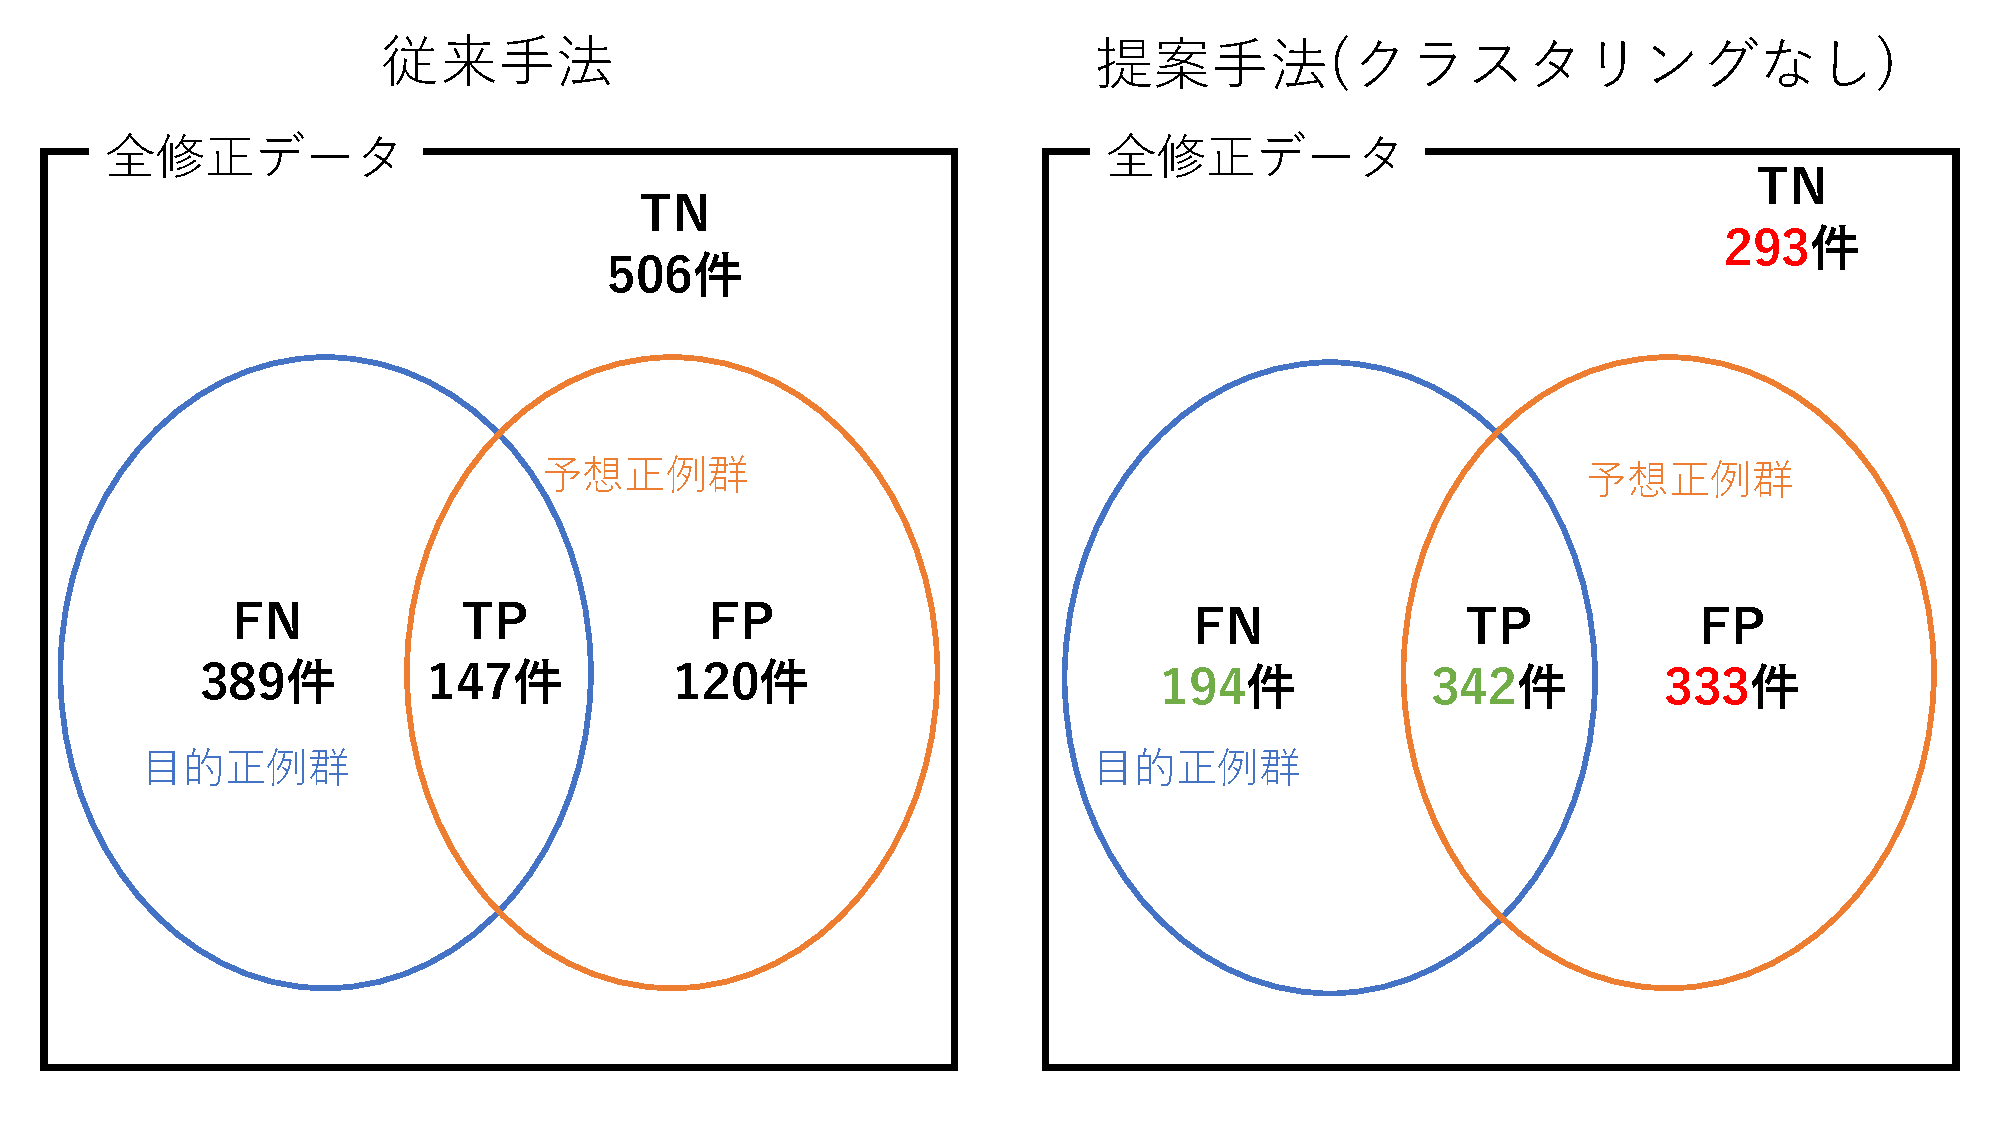
\includegraphics[width=0.25\textwidth, bb=0 0 4 3]{Kameoka_fig/benzu-schema-salad.pdf}
% 	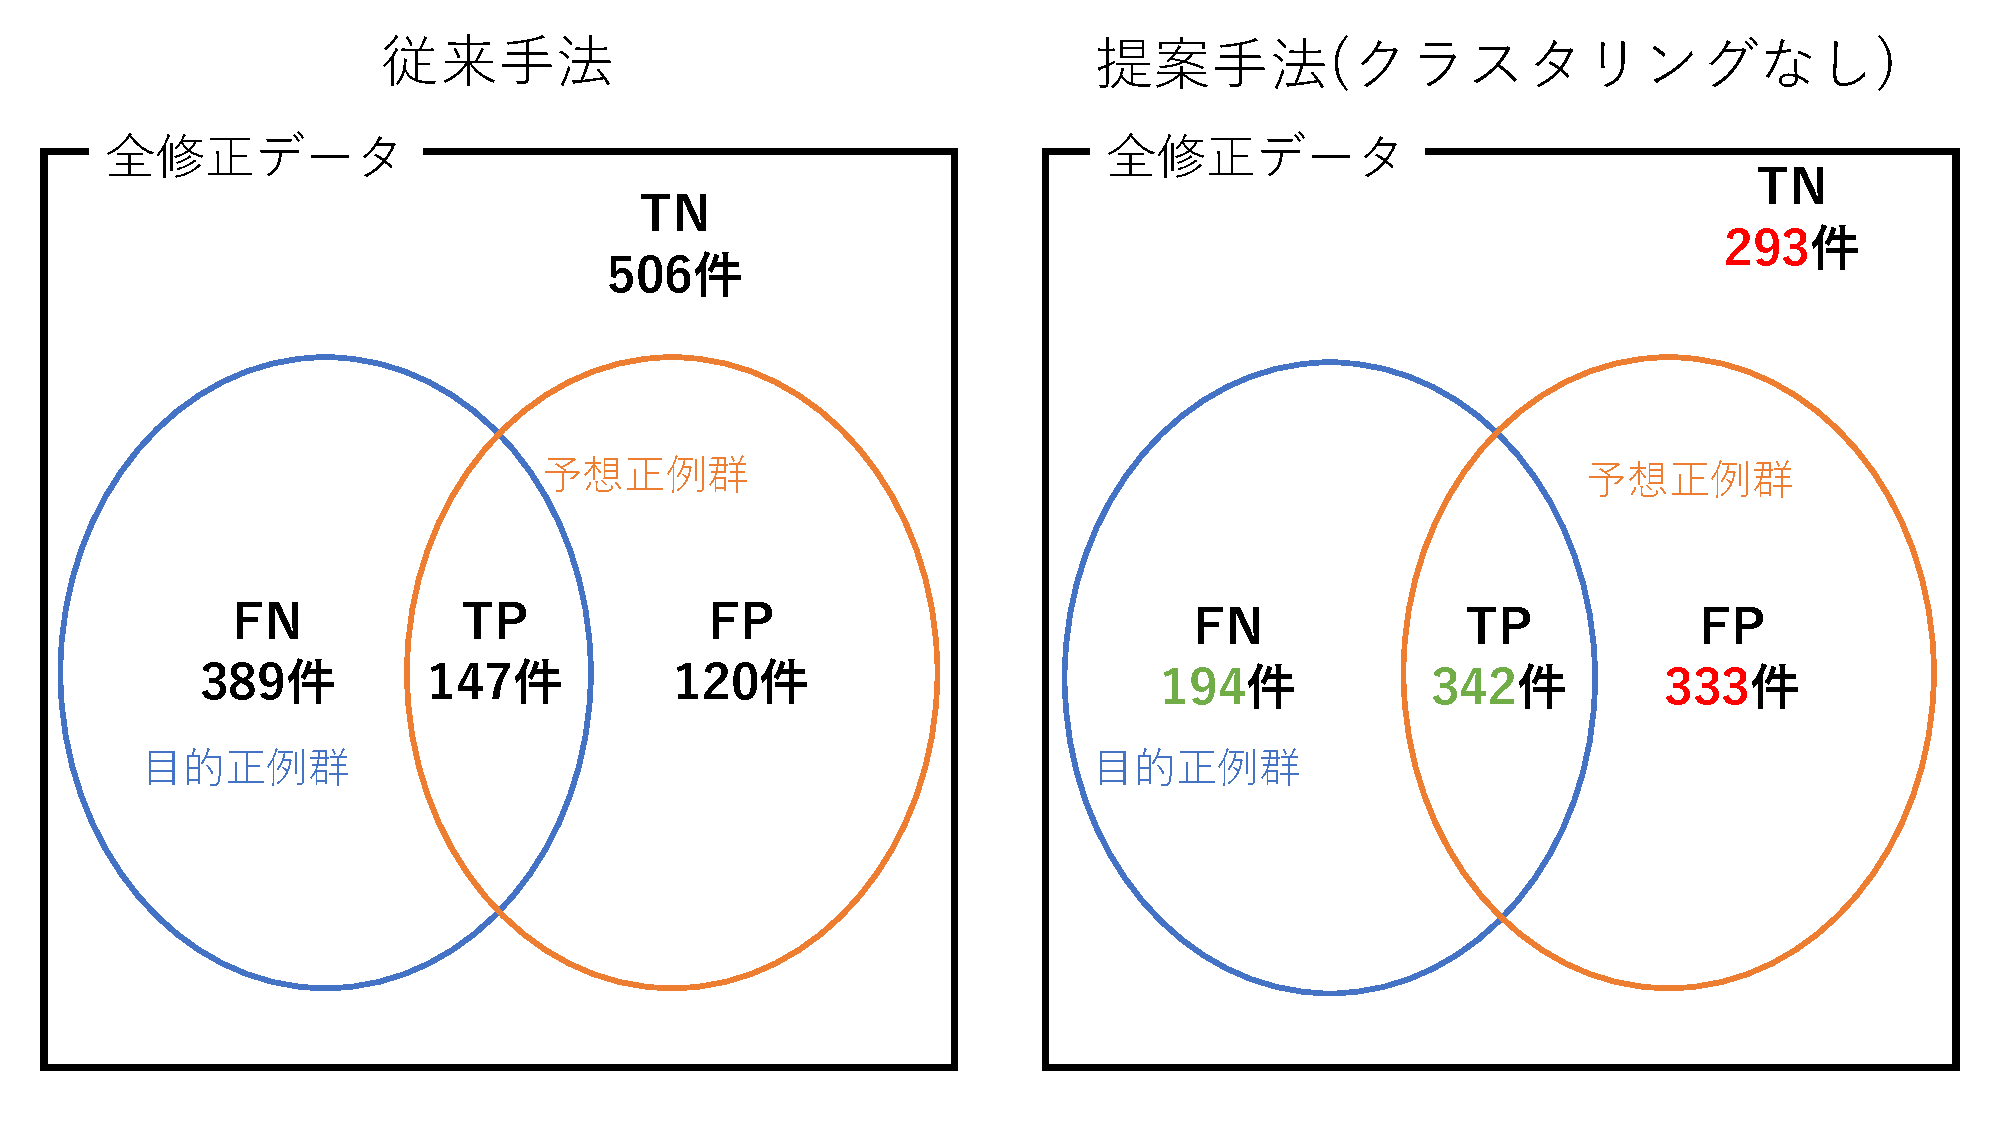
\includegraphics[width=1\linewidth]{Kameoka_fig/benzu-schema-salad.pdf}
% 	\caption{schema\_saladプロジェクトの手法ごとの予測結果のベン図}
% 	\label{fig:schema_salad}
% \end{figure}
\begin{table*}[tb]
    \centering
    \caption{ロジスティック回帰モデルで再現率とF1値が顕著に変化した予測結果}
    \vspace{2mm}
    \label{tab:log-super}
    \scalebox{0.75}{
        \begin{tabular}{l|p{4em}p{4em}p{4em}|p{4em}p{4em}p{4em}|p{4em}p{4em}p{4em}}
            \hline
            \multirow{3}{*}{プロジェクト名}&\multicolumn{3}{c|}{\multirow{2}{*}{従来手法}} & \multicolumn{3}{c|}{提案手法} & \multicolumn{3}{c}{提案手法}\\
            &\multicolumn{3}{c|}{} & \multicolumn{3}{c|}{(クラスタリングなし)} & \multicolumn{3}{c}{(クラスタリングあり)}\\ \cline{2-10}
            & \multicolumn{1}{c}{適合率} & \multicolumn{1}{c}{再現率} & \multicolumn{1}{c|}{F1値} & \multicolumn{1}{c}{適合率} & \multicolumn{1}{c}{再現率} & \multicolumn{1}{c|}{F1値} & \multicolumn{1}{c}{適合率} & \multicolumn{1}{c}{再現率} & \multicolumn{1}{c}{F1値} \\ \hline
            schema\_salad & \multicolumn{1}{r}{0.55} & \multicolumn{1}{r}{0.27} & \multicolumn{1}{r|}{0.37} & \multicolumn{1}{r}{0.51} & \multicolumn{1}{r}{0.64} & \multicolumn{1}{r|}{0.56} & \multicolumn{1}{r}{0.55} & \multicolumn{1}{r}{0.54} & \multicolumn{1}{r}{0.54} \\
            % serverless-application-model & \multicolumn{1}{r}{0.76} & \multicolumn{1}{r}{0.45}& \multicolumn{1}{r|}{0.57} & \multicolumn{1}{r}{0.55} & \multicolumn{1}{r}{0.83} & \multicolumn{1}{r|}{0.66} & \multicolumn{1}{r}{0.64} & \multicolumn{1}{r}{0.83} & \multicolumn{1}{r}{0.72} \\
            transitions & \multicolumn{1}{r}{0.83} & \multicolumn{1}{r}{0.92} & \multicolumn{1}{r|}{0.87} & \multicolumn{1}{r}{0.67} & \multicolumn{1}{r}{0.61} & \multicolumn{1}{r|}{0.64} & \multicolumn{1}{r}{0.63} & \multicolumn{1}{r}{0.86} & \multicolumn{1}{r}{0.73} \\ \hline
            % django-fsm & \multicolumn{1}{r}{0.62} & \multicolumn{1}{r}{0.99} & \multicolumn{1}{r|}{0.76} & \multicolumn{1}{r}{0.57} & \multicolumn{1}{r}{0.76} & \multicolumn{1}{r|}{0.65} & \multicolumn{1}{r}{0.60} & \multicolumn{1}{r}{0.76} & \multicolumn{1}{r}{0.67} \\ \hline
        \end{tabular}
    }
\end{table*}

\begin{table}[tb]
    \label{tab:schema_salad}
    \centering
    \caption{schema\_saladプロジェクトの手法ごとの予測結果の混合行列}
    \vspace{2mm}
    \begin{tabular}{ll|r|r||r|r}
    \hline
        ~ & ~ & \multicolumn{4}{c}{予測結果} \\ \cline{3-6}
        ~ & ~ & \multicolumn{2}{c||}{従来手法} & \multicolumn{2}{c}{提案手法} \\ \cline{3-6}
        & ~ & 0 & 1 & 0 & 1 \\ \hline
        \multirow{2}{*}{実データ} & \multicolumn{1}{|c|}{0} & 506 & 120 & 293 & 333\\ \cline{2-6}
        & \multicolumn{1}{|c|}{1} & 389 & 147 & 194 & 342\\ \hline
    \end{tabular}

    \vspace{4mm}
    \centering
    \label{tab:transitions}
    \caption{transitionsプロジェクトの手法ごとの予測結果の混合行列}
    \vspace{2mm}
    \begin{tabular}{ll|r|r||r|r}
    \hline
        ~ & ~ & \multicolumn{4}{c}{予測結果} \\ \cline{3-6}
        ~ & ~ & \multicolumn{2}{c||}{従来手法} & \multicolumn{2}{c}{提案手法} \\ \cline{3-6}
        & ~ & 0 & 1 & 0 & 1 \\ \hline
        \multirow{2}{*}{実データ} & \multicolumn{1}{|c|}{0} & 86 & 45 & 58 & 73 \\ \cline{2-6}
        & \multicolumn{1}{|c|}{1} & 20 & 217 & 92 & 145 \\ \hline
    \end{tabular}
\end{table}


% \begin{figure}[bp]
% 	\centering
%     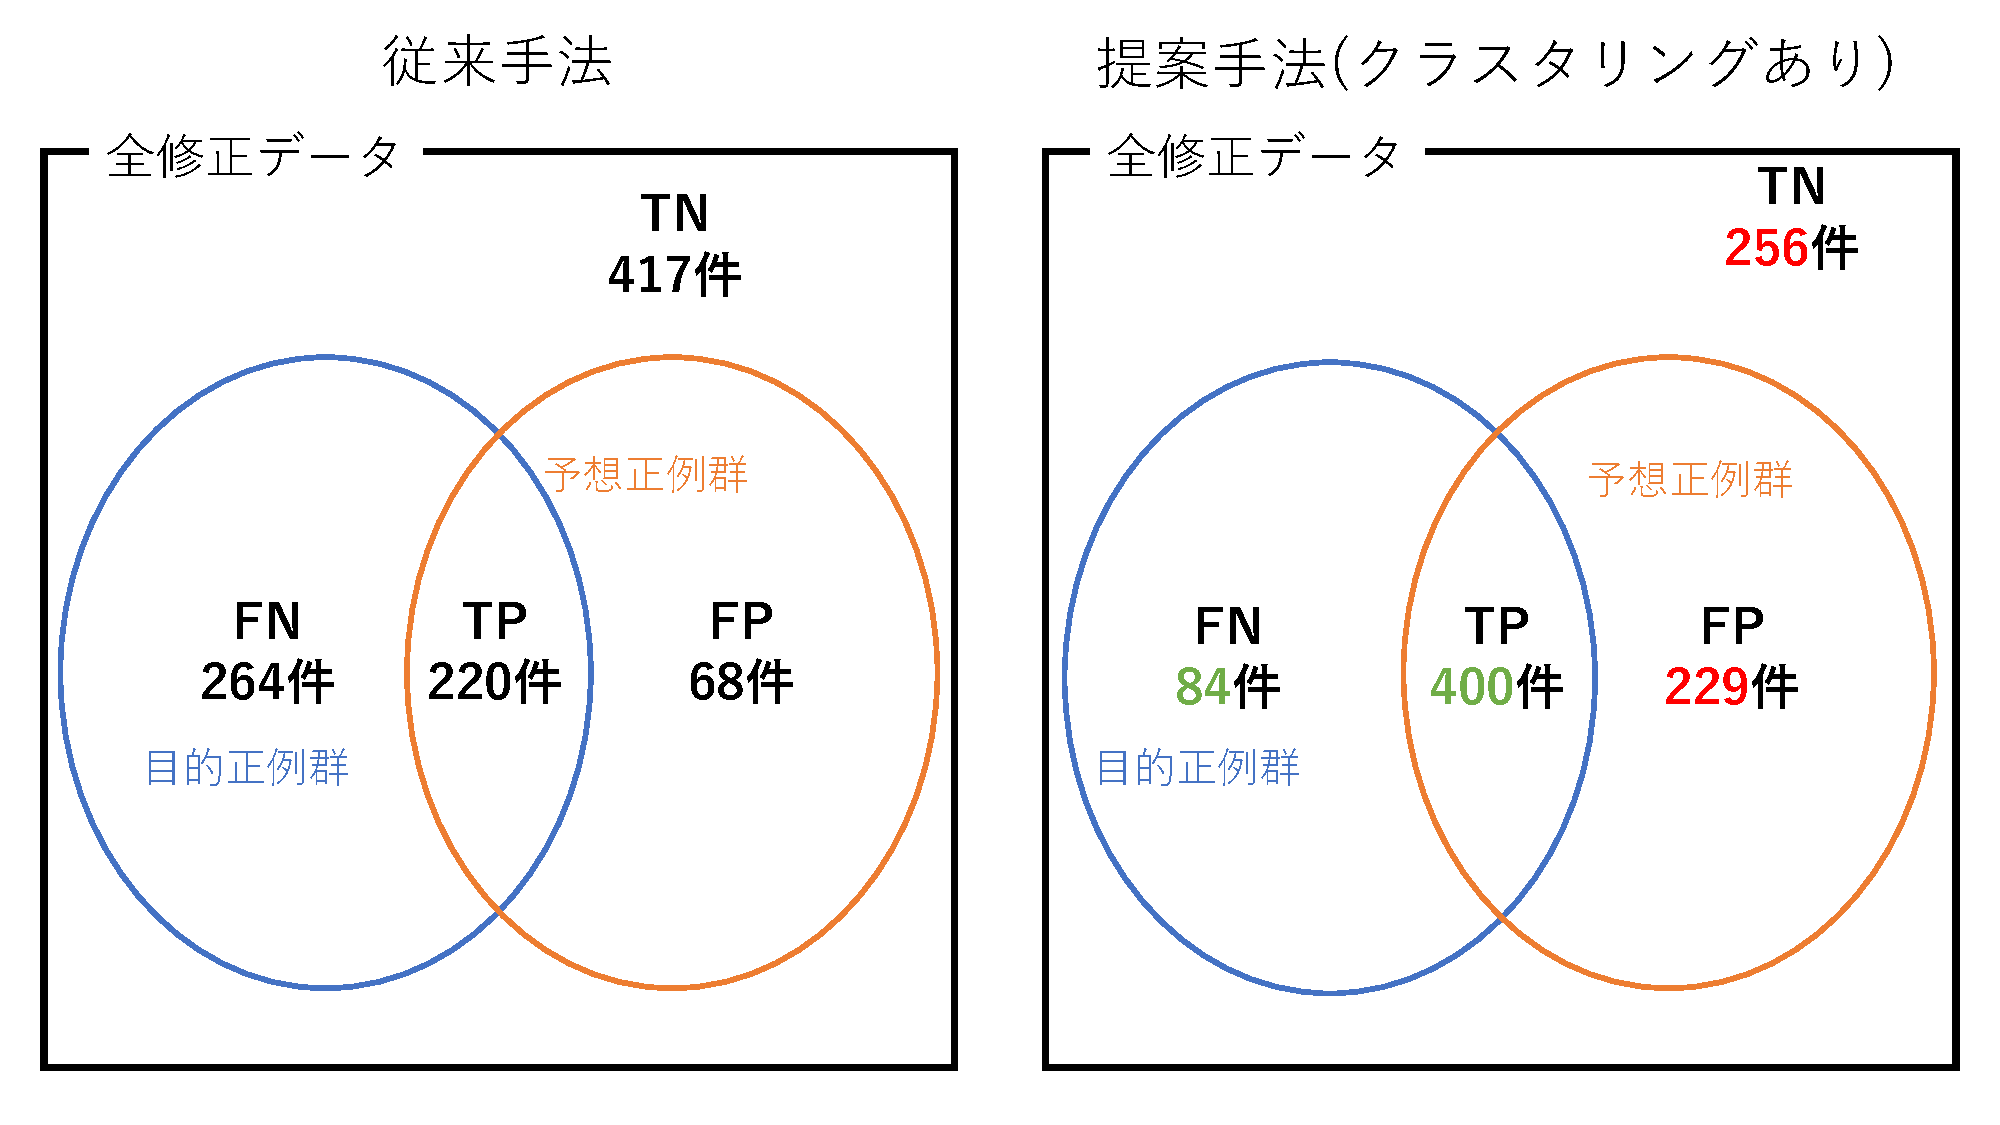
\includegraphics[width=0.25\textwidth, bb=0 0 4 3]{Kameoka_fig/benzu-serverless-application-mode.pdf}
% 	% 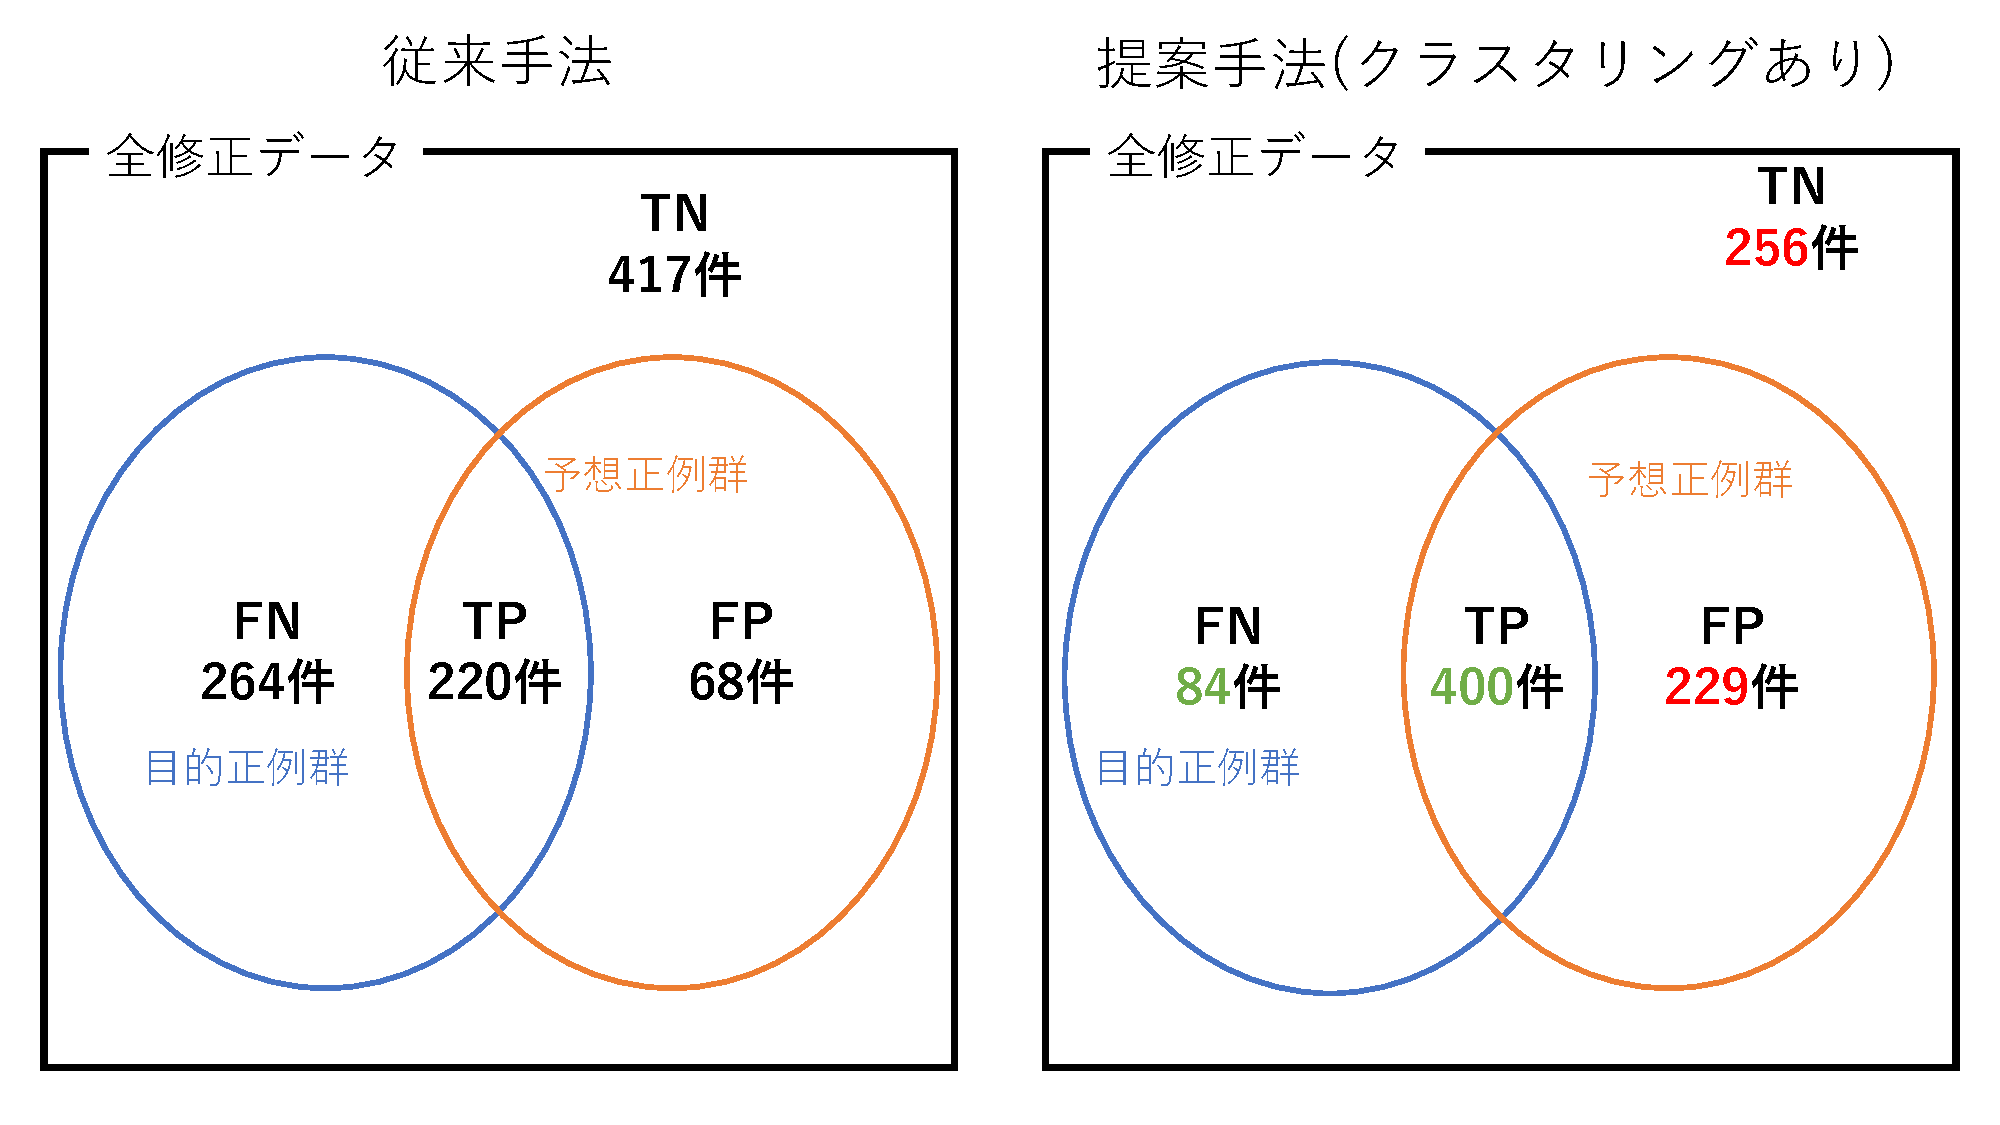
\includegraphics[width=1\linewidth]{Kameoka_fig/benzu-serverless-application-mode.pdf}
% 	\caption{serverless-application-modeプロジェクトの手法ごとの予測結果のベン図}
% 	\label{fig:serverless-application-mode}
% \end{figure}



%\begin{figure}[tb]
% 	\centering
%     % 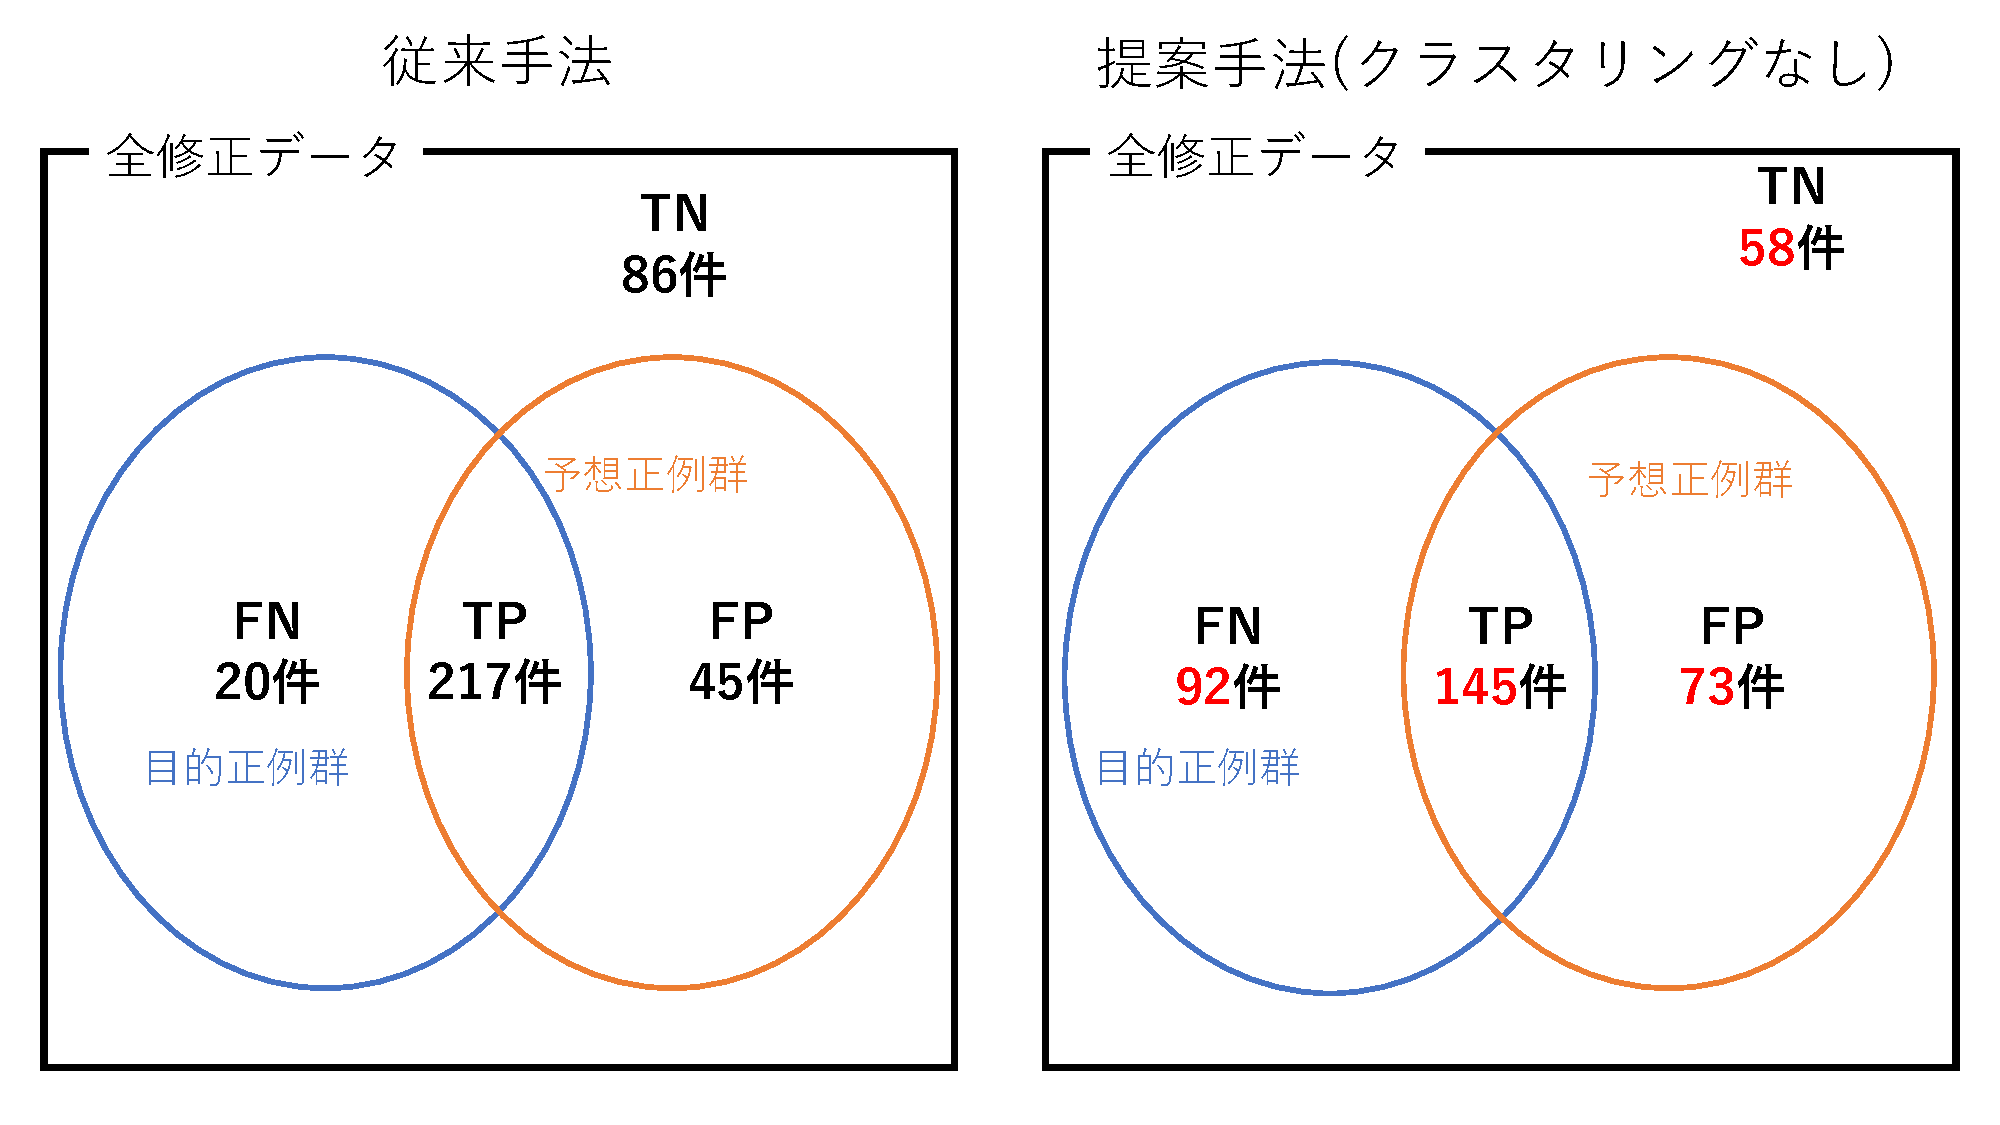
\includegraphics[width=0.25\textwidth, bb=0 0 4 3]{Kameoka_fig/benzu-transitions.pdf}
% 	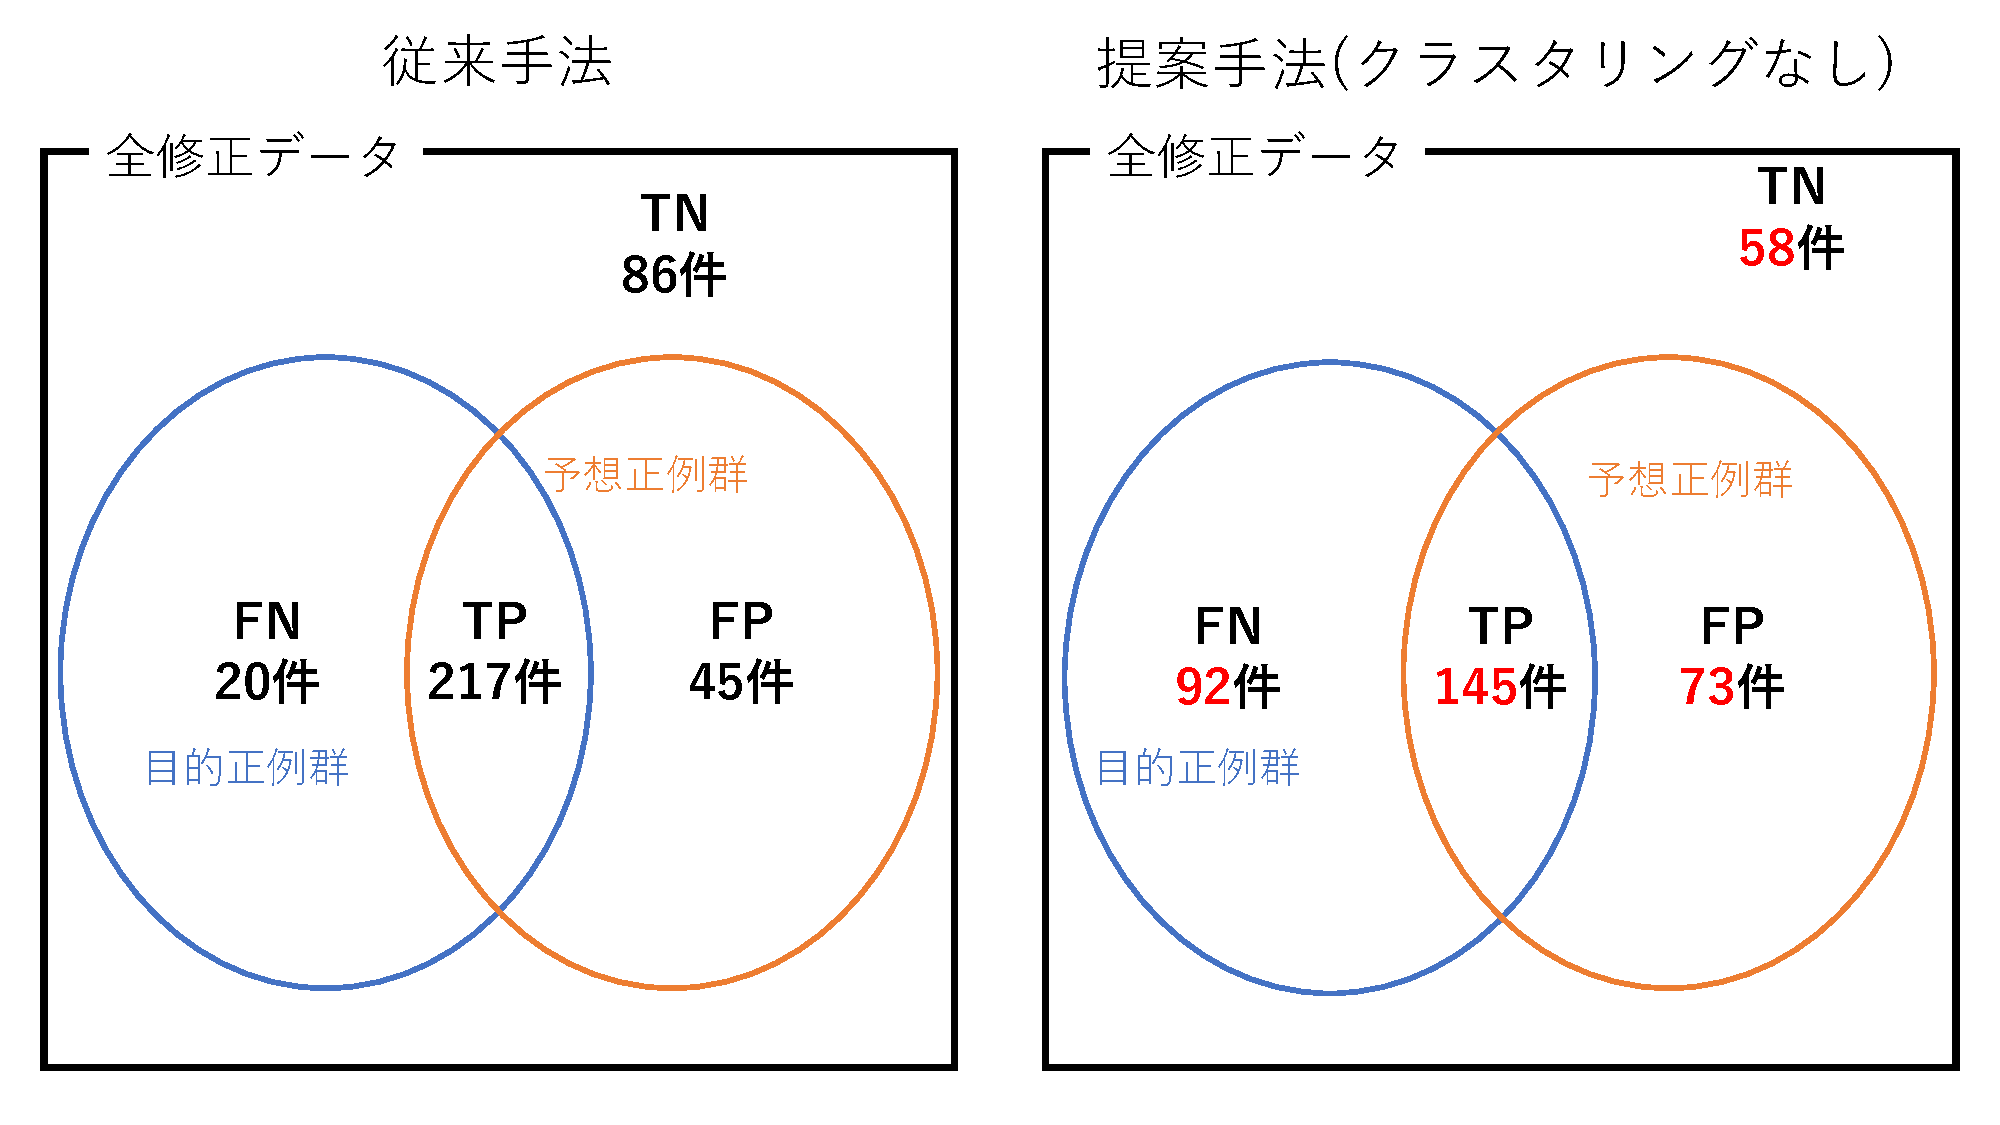
\includegraphics[width=1\linewidth]{Kameoka_fig/benzu-transitions.pdf}
% 	\caption{transitionsプロジェクトの手法ごとの予測結果のベン図}
% 	\label{fig:transitions}
% \end{figure}

% \begin{figure}[bp]

% 	\centering
%     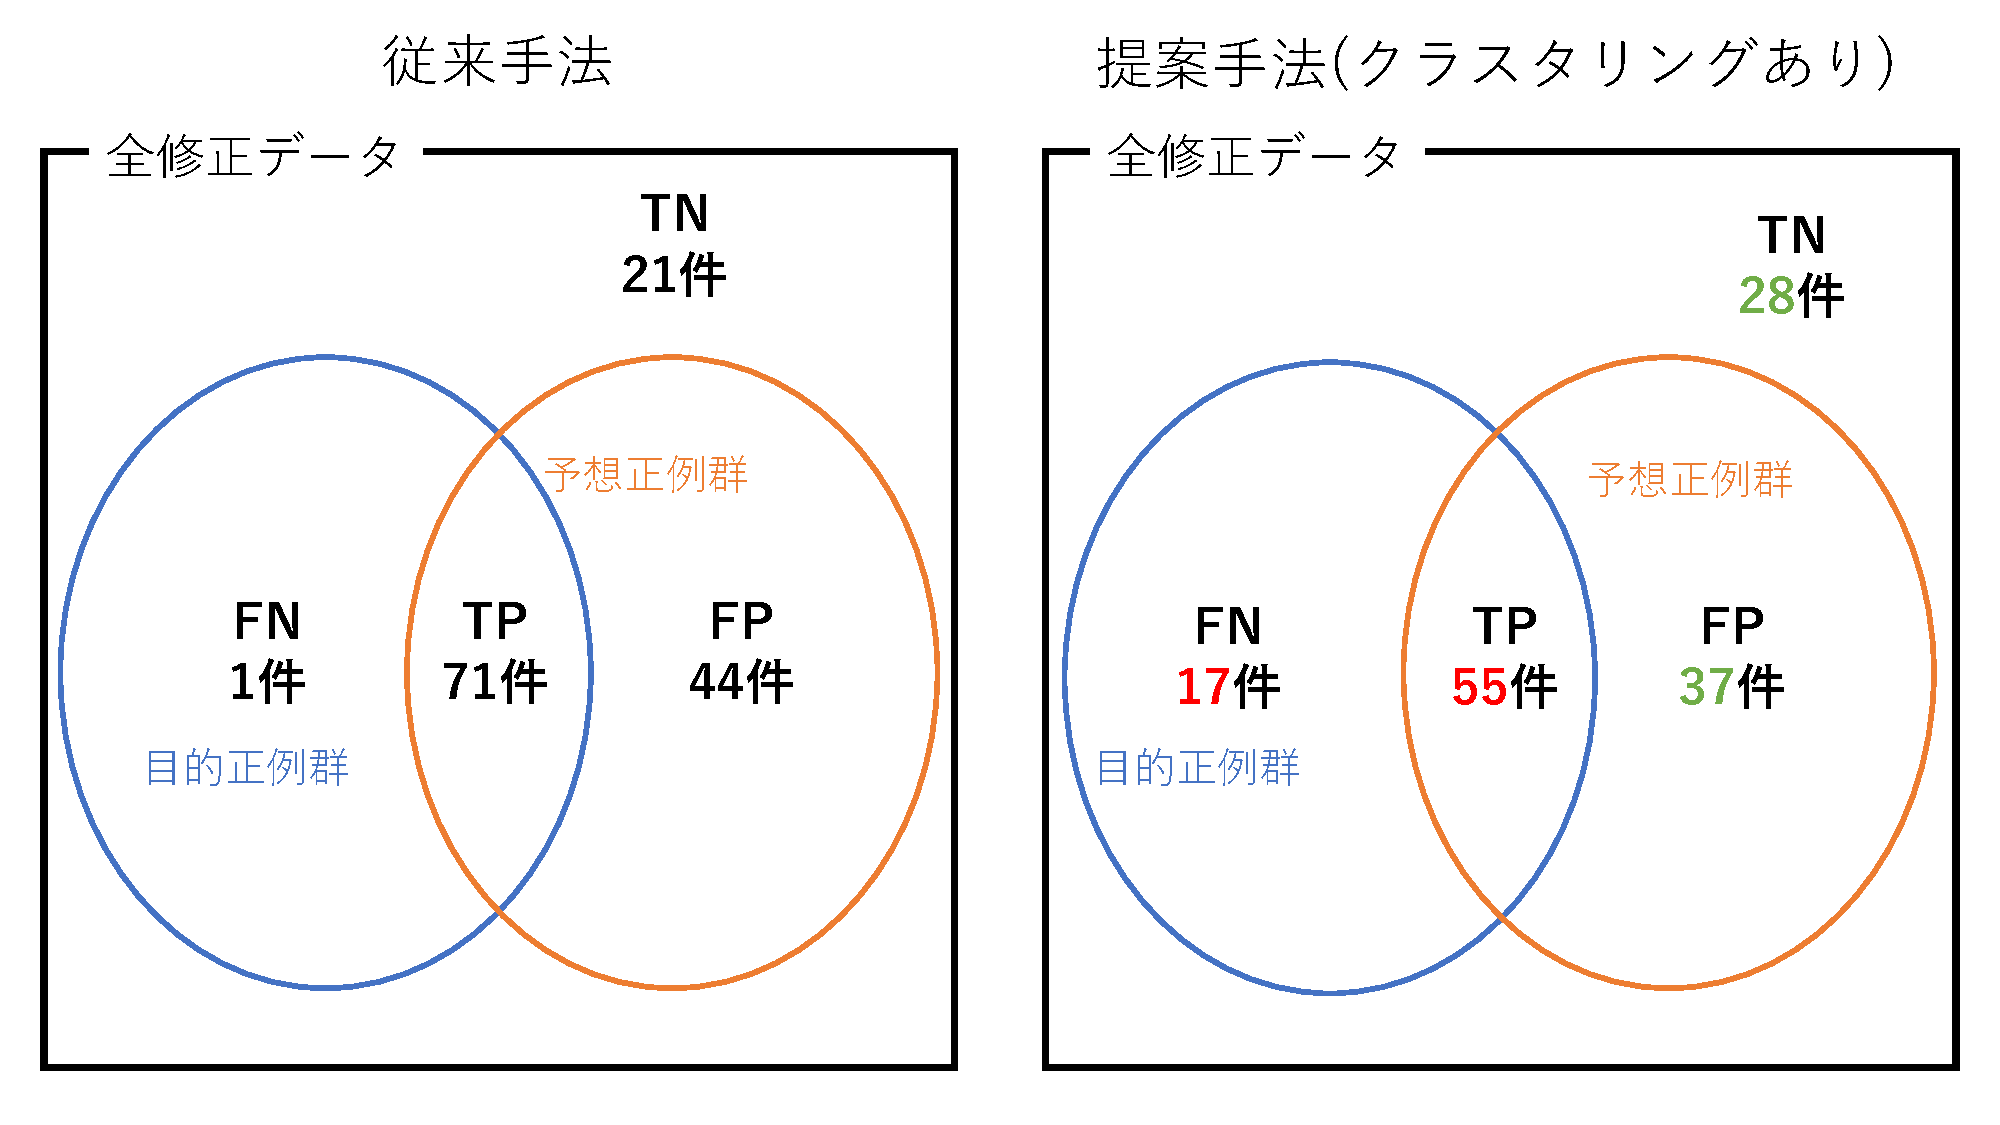
\includegraphics[width=0.25\textwidth, bb=0 0 4 3]{Kameoka_fig/benzu-django-fsm.pdf}
% 	% 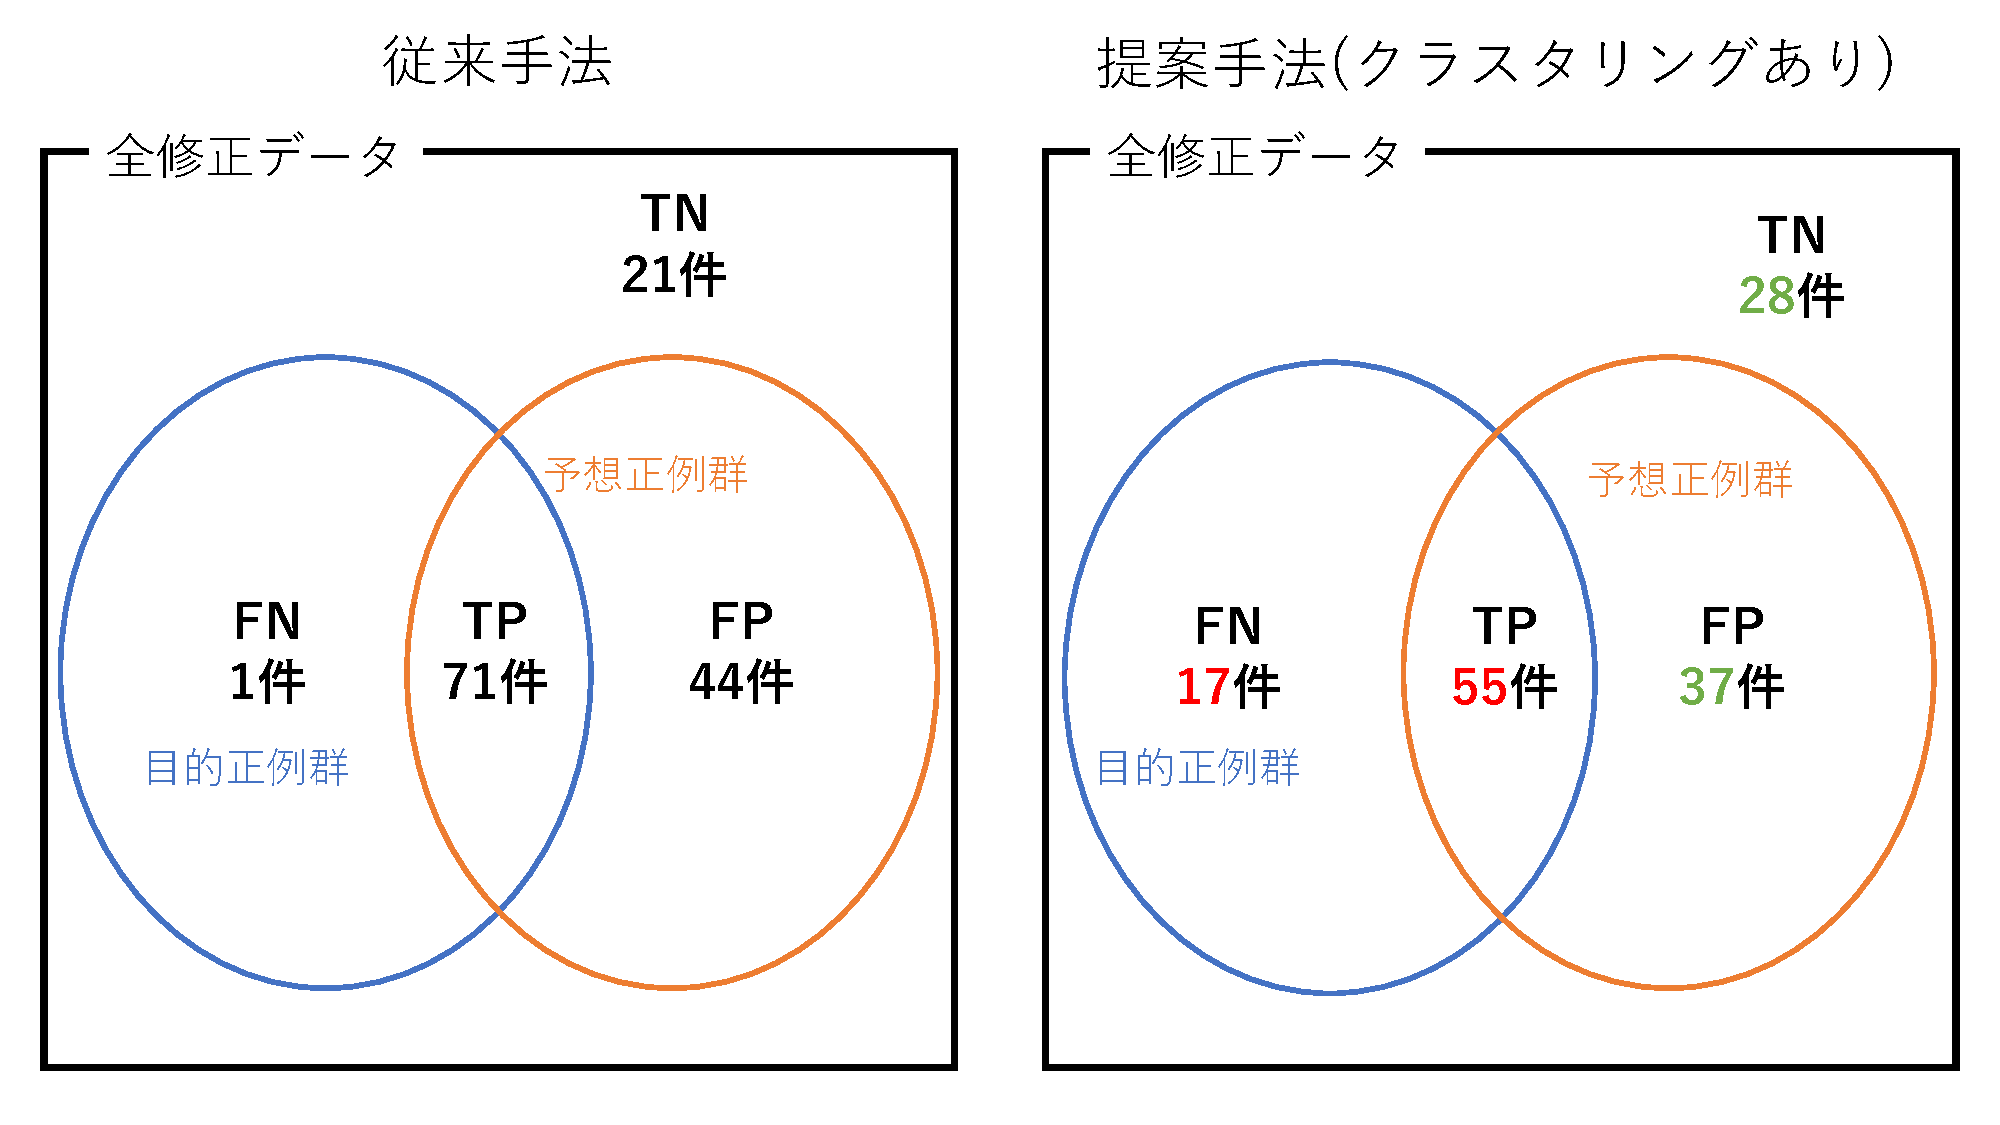
\includegraphics[width=1\linewidth]{Kameoka_fig/benzu-django-fsm.pdf}
% 	\caption{django-fsmプロジェクトの手法ごとの予測結果のベン図}
% 	\label{fig:django-fsm}
% \end{figure}

RQ1の結果から,提案手法でデータセットを拡張したことによって,検出されたコーディング規約違反が修正されると予測した正例データが増加し,再現率が向上し,適合率が低下したことが示唆された.
本章では,従来手法と提案手法の具体的な予測結果について分析する.分析を行う対象として,RQ1において提案手法によって予測精度が顕著に変化したプロジェクトを分析対象とする.
% ここで,プロジェクトを選択して分析を行うのは,従来手法と提案手法との予測結果の違いが顕著なプロジェクトを分析することで,提案手法の有効性を確認するためである.

表\ref{tab:log-super}はロジスティック回帰モデルを用いた提案手法によって予測精度が大きく変化したプロジェクトの予測結果から2プロジェクトを抜粋したものである.ロジスティック回帰モデルの結果を抜粋した理由としては,2種類のアルゴリズムの中で提案手法によってより精度に大きな変化が見られたからである.
schema\_saladプロジェクトは提案手法によって予測精度が向上し,2行目のtransitionsプロジェクトは提案手法によって予測精度が低下した結果である.
% 表\ref{tab:log-super}に記載した提案手法によって予測精度が向上した2プロジェクト,提案手法によって予測精度が低下した2プロジェクトにおける修正予測結果について分析を行う.

表6,表7はschema\_saladとtransitionsプロジェクトの予測結果の混合行列を示す.表の左半分は従来手法の結果を示し,右半分は提案手法(クラスタリングなし)の結果を示す.
各混合行列の左上はTNの数を示し,右上はFPの数を示し,右下はTPの数を示し,左下はFNの数を示している.
% 各混合行列の左上は実際には修正されなかった違反を修正されないと正しく予測できたTNを表す.右上は,実際には発生した違反が修正されなかったが,誤って修正されると予測したFPを表す.右下は,発生した違反が実際に修正され,予測でも正しく修正されると予測できたTPの数を表す.左下は実際に修正された違反を誤って修正されないと予測したFNの数を表す.

% 図\ref{fig:schema_salad}と図\ref{fig:transitions}に従来手法と提案手法(クラスタリングなし)または,従来手法と提案手法(クラスタリングあり)の予測結果をベン図にまとめる.図中のベン図は,プロジェクトで検出された全コーディング規約違反データの内,左側の円で囲われたものが目的変数の正例群を示し,右側の円は予測結果の正例群を示している.両方の円で囲まれた部分は実データと予測結果が共に正例であるためTPの違反修正箇所数を示し,左円のみに囲まれている部分は,予測できなかった正例であるためFNの修正箇所数を示し,右円のみに囲まれている部分は誤って正例と予測したためFPの修正箇所数を示し,どちらにも囲まれていない部分は,実際に修正されず予測でも修正されないと予測したためTNの修正箇所数を表している.\todo{混合行列を表で書いては?}

\subsubsection{提案手法によって予測可能・不可能になったコーディング規約違反とは?}
% \done{答えがない}
% \subsubsection*{分析1 提案手法によって予測可能になったコーディング規約違反とは?\todo{答えがない}}

表6のschema\_saladプロジェクトの予測結果から,提案手法(クラスタリングなし)によって再現率が向上しており,適合率が低下していることがわかる.
適合率は0.55から0.51(0.93倍)に低下し,再現率は0.27から0.64(2.37倍)に向上した.
% 提案手法(クラスタリングなし)の予測結果は従来手法からの再現率の上昇率が,適合率の低下率を上回る場合,適合率と再現率の両方を考慮した指標のF1値が向上する.
具体的な予測結果をコーディング規約ごとに分析すると,多くのコーディング規約で提案手法によって正しく予測できている数が増加していることが確認できた.
また,W1406(不必要なプレフィックスがついている)の規約では従来手法では全73件中19件しか正解していなかったが,提案手法では正解数が67件まで大幅に増加している.W1406以外にも提案手法によって正解数が大幅に増加している規約が見られた.
提案手法によって正解数が大幅に増加している規約は,従来手法と提案手法で共通して正解している規約より学習データが少ない傾向にあることが確認できた.
したがって,提案手法によって予測が可能になるコーディング規約違反は,学習データに存在する数が少なく,複数プロジェクトのデータによって学習データを拡張できるコーディング規約であることを明らかにした.

% \subsubsection*{分析2 提案手法によって余剰に正例として予測したコーディング規約違反とは?\todo{答えがない}}

表7に提案手法によって予測精度が低下した場合の予測結果の内訳を示す.
transitionsプロジェクトは従来手法によってTPが217件から145件に減少し,TNも86件から58件に低下している.
具体的な予測結果を分析すると,transitionsプロジェクトはテストデータにC0116(関数またはメソッドにdocstringが無い)の規約が22件含まれており,従来手法では22件すべて正解しているが,提案手法では8件しか正解していない.これは,C0116へのtransitionsプロジェクトの修正傾向が他プロジェクトの傾向と異なるからであると考えられる.他のコーディング規約も同様に,テストデータに多数含まれており,従来手法では正しく予測できているが,提案手法では予測できていないコーディング規約が散見される.テストデータに多数含まれているコーディング規約は,学習用データにも多数含まれていることが多い.つまり,提案手法によって予測不可能になる規約違反は,単一プロジェクトで頻出しているコーディング規約で,他プロジェクトの修正方針と異なるコーディング規約への違反である.


% \subsubsection{結果のまとめ}

% 提案手法(クラスタリングなし),提案手法(クラスタリングあり)によって予測精度が向上しているプロジェクトでは,データセットを拡張したことによってTPが増加,FNが減少したことによる再現率の向上と,それに伴うF1値の向上によって従来手法を上回る予測精度でコーディング規約違反の修正予測が可能となった.しかし,従来手法によって高い精度で予測できているものは,提案手法によってTPが減少する場合や,FPがTPの増加より上回って増加してしまう場合は再現率が低下しF1値も低下する.

%%%%%%%%%%%%%%%%%%%%%%%%%%%
\section{考察}\label{chap:consideration}
%%%%%%%%%%%%%%%%%%%%%%%%%%%

\subsection{RQの結果からなぜ提案手法によって再現率が向上したのか}\label{kosatu}

RQ1の結果では提案手法の再現率が従来手法に比べて向上し,F1値も向上することが明らかになった.
その理由は,RQ2の結果から,従来手法は正例として予測できなかったコーディング規約違反の修正予測が,提案手法によって可能になったためである.
また,提案手法を用いることによって,従来手法では予測ができなかった正例を正しく予測できるようになったことは,複数プロジェクトを学習し,単一プロジェクトでは十分に学習できなかったコーディング規約について学習ができたためであると考えられる.
本研究ではPylintのコーディング規約の種類をone-hotベクトル化して説明変数として利用している.
そのため,単一プロジェクトにおいて低頻度でしか発生しないコーディング規約違反は予測において規約の種類に適切なパラメータを学習することが困難であるため,誤った予測をしてしまうと考えられる.

コーディング規約を種類ごとにone-hotベクトル化している点は,単一プロジェクトで頻出しているコーディング規約違反があった場合に,単一プロジェクトで的確な重みづけができていたものを,複数プロジェクトのコーディング規約が結合されたことによって,重みづけが汎化され予測精度に悪影響を及ぼすことが考えられる.本研究で追加分析したところ,図\ref{fig:importance}のような結果が得られた.図中の表はロジスティック回帰による各モデルの重要度の絶対値を降順に10個表示している.左右の表は従来手法によるモデルで,左表は本手法で精度が向上したschema\_saladプロジェクトを示し,右表は本手法で精度が低下したtransitionsプロジェクトの結果を示す.中表は提案手法のすべてのプロジェクトのデータを結合したモデルの結果を示す.要素同士を繋ぐ実線はモデル間で重要度の高い10個で共通していることを示し,点線は提案モデルの重要度の高い10個以外と繋がっている.
予測精度が低下したtransitionsプロジェクトでは,図\ref{fig:importance}で提案モデルと実線で繋がれているものが1個のみであり,他プロジェクトに比べて違反している規約に特徴があることがわかる.そのため,単一プロジェクトのデータを学習することで,特徴を捉えたモデルを構築できていたが,大多数のデータによって特徴が打ち消されたことがわかる.
予測結果の向上したschema\_saladプロジェクトで違反している規約は,図\ref{fig:importance}で実線で繋がれているものが5個あり,他プロジェクトで発生している違反と同じものが多く,複数プロジェクトのデータを学習に用いることによって予測精度が向上したと考えられる.

本研究では,コーディング規約の修正予測において,複数プロジェクトの開発データを学習に用いることによって予測精度が向上するプロジェクトが68プロジェクトの半数程度存在することが明らかになった.今後提案手法が有効に働くプロジェクトの特徴を明らかにすることによって,本研究の提案手法を適用する場面が明確になると考えられる.

\subsection{提案手法(クラスタリングあり)の有効性とは}

\begin{table*}[tb]
    \centering
    \caption{クラスタごとの予測結果の分析}
    \label{tab:cluster}
    \vspace{1mm}
    \scalebox{0.80}{
        \begin{tabular}{l|p{3em}|p{3em}|p{3em}|p{3em}|p{3em}|p{3em}|p{3em}|p{3em}|p{3em}|p{3em}}
        \hline
        cluster & \hfill 01 & \hfill 02 & \hfill 03 & \hfill 04 & \hfill 05 & \hfill 06 & \hfill 07 & \hfill 08 & \hfill 09 & \hfill 10 \\ \hline
        適合率 & \hfill 0.34 & \hfill 0.09 & \hfill 0.57 & \hfill 0.47 & \hfill 0.51 & \hfill nan & \hfill 0.00 & \hfill nan & \hfill nan & \hfill nan \\
        再現率 & \hfill 0.64 & \hfill 0.59 & \hfill 0.39 & \hfill 0.83 & \hfill 0.72 & \hfill nan & \hfill 0.00 & \hfill nan & \hfill nan & \hfill nan \\ 
        F1値 & \hfill 0.44 & \hfill 0.16 & \hfill 0.46 & \hfill 0.60 & \hfill 0.60 & \hfill nan & \hfill nan & \hfill nan & \hfill nan & \hfill nan \\ \hline
        テストデータ数 & \hfill 18,368 & \hfill 259 & \hfill 82 & \hfill 2,129 & \hfill 4,719 & \hfill 0 & \hfill 86 & \hfill 1 & \hfill 495 & \hfill 0 \\ \hline
        \end{tabular}
    }
\end{table*}

\begin{figure}[tb]
	\centering
	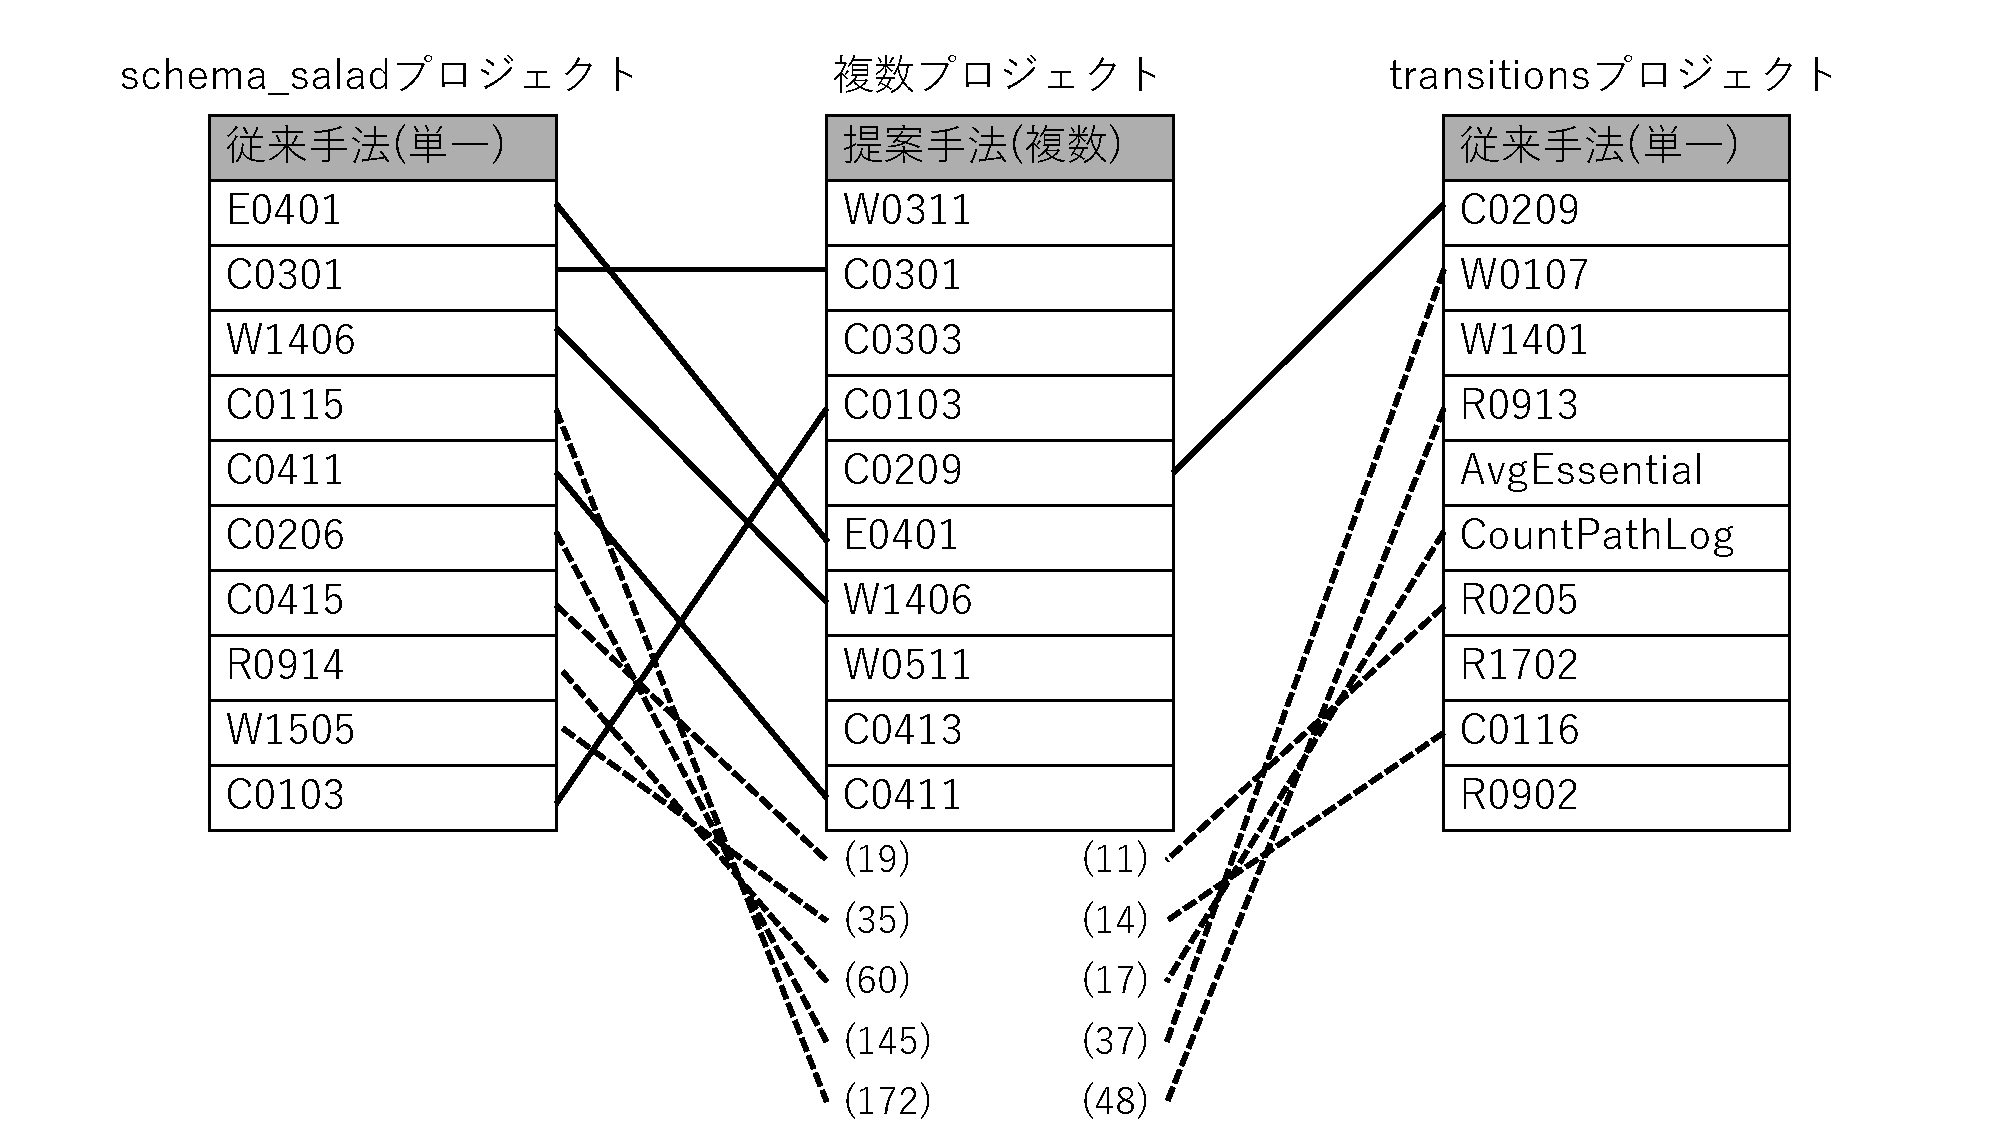
\includegraphics[width=1.0\linewidth]{Kameoka_fig/importance.pdf}
	\caption{従来モデルと提案モデルの重要度の比較}
	\label{fig:importance}
\end{figure}

提案手法として,複数プロジェクトのデータを結合した後にクラスタリングを行い,各クラスタごとにロジスティック回帰予測モデルを作成し予測を行った.クラスタリングによる予測精度の変化を分析するために,各クラスタごとの予測精度を算出した.表\ref{tab:cluster}に,各クラスタごとの予測精度を示す.表の最下列は各クラスタに分類されたテストデータ数を示している.表からわかるようにcluster06とcluster10にはテストデータが存在せず,cluster01,cluster04,cluster05に多くのデータが集まっている.表中の`nan'は予測結果をすべて負例として予測した場合に適合率,再現率,F1値が計算できずに代入される.
クラスタごとの予測結果で最もF1値が高いのはcluster04,cluster05の0.60である.また,cluster06以降では違反修正データの有無に関わらず修正予測ができていない.各クラスタごとに各評価指標の値に違いが見られるため,総違反修正データのクラスタリングが予測精度に影響を与えていることがわかる.また,cluster04,cluster05のデータ数は2,129と4,719であり,cluster01はクラスタに含まれるデータ数が過多であり,cluster02とcluster03はデータ数が過小であると考えられる.

各クラスタごとの予測精度から,クラスタリングにより抜粋された説明変数のみ学習する提案手法(クラスタリングあり)は,クラスタごとに予測精度が異なり,クラスタに含まれるデータ数が2,129と4,719の際に最大のF1値を確認したため,各クラスタに含まれるデータ数をcluster04,cluster05に近づけるようにクラスタリングを行うことによって,更なる予測精度の向上を見込むことができると考えられる.

%%%%%%%%%%%%%%%%%%%%%%%%%%%
\section{妥当性への脅威}\label{chap:heuristic}
%%%%%%%%%%%%%%%%%%%%%%%%%%%
\subsection{内的妥当性}

% 本研究で利用したデータセットは,プロジェクトごとの規約修正履歴の期間は統一して収集しているが,複数プロジェクトを結合して学習した場合には予測地点では得られない他プロジェクトの未来のデータを学習している.複数プロジェクトのデータを学習し,予測する際にも時系列を考慮することは今後の課題である.

目的変数の計測において,規約違反しているコードが修正された場合のみ正例として扱い,削除された場合は,修正されたわけではないため本研究では負例として扱っている.しかし,コーディング規約違反の中には該当部分を削除することによっても解消するものがあるため,本来正例として扱うべきケースを負例として計測してしまっていることがある.
また,目的変数の計測は一様に最終リビジョンにおいて,コーディング規約違反が修正されたか否かで計測しており,違反の発生地点は考慮していない.つまり,最終リビジョンの一つ前のリビジョンで発生した違反と,最初のリビジョンで発生した違反を同等に扱っているため,最終リビジョンに近いほど修正までの猶予が短いことを考慮していない.

% 本研究では2値分類機械学習アルゴリズムとして,ロジスティック回帰,RandomForest,SVMの3種類のアルゴリズムを用いて検出されたコーディング規約違反の修正予測を行った.結果として,RandomForestが最も高い精度で予測し,SVMが最も低い精度での予測結果となった.
本研究で用いた2種類の機械学習アルゴリズム以外にも、より正確な予測を可能にするアルゴリズムが存在する可能性がある.
それぞれのパラメータの更新回数である,イテレーション回数を10,000に設定したが,データサイズが大きいプロジェクトではモデルが収束しないことが確認された.モデルが収束しない場面も確認されたが,本研究で主に用いた実験環境とは別の環境で,複数回実行した場合でも予測結果に変化はなかったので,モデルが収束しない問題に関しては,本研究の結果に対して大きな影響を与える可能性は低い.

% 提案手法で説明変数の階層的クラスタリングを行う際に,クラスタ間の連結法にはWard法を用い,距離の測定にはユークリッド距離を用いた.連結法や距離の測定方法にはPython言語のライブラリであるsklearnのAgglomerativeClusteringパッケージ
% % \footnote{sklearn.cluster.AgglomerativeClustering: \\\url{https://scikit-learn.org/stable/modules/generated/}\allowbreak\url{sklearn.cluster.AgglomerativeClustering.html}}
% のデフォルト値を使用している.階層的クラスタリングする際の連結法や距離の測定方法を変えることによって,各データが属するクラスタが変化すると考えられるが,本研究でのクラスタリングの結果では,大多数のデータが集まるクラスタと,そうでないクラスタに二極化したため,連結法と距離の測定方法による結果への影響は小さいと考えられる.

\subsection{外的妥当性}

本研究ではケーススタディとしてPython言語を主な開発言語としたプロジェクト68件の規約違反修正履歴を収集して検証を行った.
また,プロジェクト数をさらに拡張した場合や,対象とするプロジェクトや期間を変更した場合に予測精度が変化することが示唆される.
対象言語をPython以外の言語とした場合予測結果が変化することが示唆される.
しかし,本研究で使用したデータセットは68プロジェクトでプロジェクトごとのデータ数が中央値で500.5件のデータ数を含んでいるので,更なるデータサイズの拡張による予測精度への影響は低いと考えられる.

%%%%%%%%%%%%%%%%%%%%%%%%%%%
\section{おわりに}\label{chap:end}
%%%%%%%%%%%%%%%%%%%%%%%%%%%

本研究では,静的解析ツールによってソースコード中に含まれるコーディング規約違反を検出した結果から,修正すべき違反か否かに分類するタスクにおいて予測対象プロジェクト以外の開発データも予測モデルの学習に用いた場合の予測結果への影響を調査した.結果として,ロジスティック回帰モデル,RandomForestモデルの2種類のモデル構築手法において,従来手法である予測対象プロジェクトの過去の規約違反修正履歴のみを学習した場合が,提案手法より多いプロジェクトで高いF1値で修正予測が可能であった.しかし,予測対象プロジェクト以外の開発データも学習する提案手法(クラスタリングなし),提案手法(クラスタリングあり)によって検証に使用した68プロジェクトの1/4程度ずつのプロジェクトでF1値の向上を確認した.
F1値が向上した理由として,データセットを拡張したことによる,モデルの最適化によって予測精度が向上したことが示唆される.しかし,違反しているコーディング規約の種類が他プロジェクトに比べて特徴的な場合,不必要なデータを学習してしまい,予測精度が低下することも確認した.

本研究において複数プロジェクトを学習に用いる提案手法によって予測精度が向上するプロジェクトを確認することができたので,各プロジェクトごとに違反しているコーディング規約の特徴ごとにグループ化し,各グループごとに学習することによって,コーディング規約違反の修正予測精度の向上を見込むことができる.

\bibliographystyle{junsrt}
\bibliography{Kameoka}

\end{document}
